\documentclass[alpha-refs]{wiley-article}

\usepackage[binary-units]{siunitx}
\usepackage{bm,bbm}
\usepackage{booktabs}
\usepackage{subfig}
\usepackage{float}
\usepackage{rotating}
\graphicspath{{./Figures/}}
\usepackage[linesnumbered,lined,boxed]{algorithm2e}
\makeatletter
\renewcommand{\@algocf@capt@plain}{above}% formerly {bottom}
\makeatother
\usepackage{undertilde}

\usepackage{todonotes}
\usepackage{comment}   

\DeclareSIUnit{\minusalphapercent}{(1-\alpha)\%}
\DeclareSIUnit{\alphapercent}{\alpha\%}

\newcommand{\Mycite}[1]{%
 (\citeauthor{#1},~\citeyear{#1})}

\papertype{Original Article}

\title{Time Series Analysis with Bandt \& Pompe Symbolization and a Test for White Noise in the Entropy-Complexity Plane}

\abbrevs{RNG, random number generator; PRNG, pseudorandom number generator; TWNRS, true white noise random sequence.}

\author[1]{Eduarda T.\ C.\ Chagas}
\author[2,3]{Marcelo Queiroz-Oliveira}
\author[4]{Osvaldo A.\ Rosso}
\author[1]{Heitor S.\ Ramos}
\author[2]{\mbox{Cristopher G.\ S. Freitas}}
\author[5]{Alejandro C.\ Frery}

\contrib[]{All authors contributed equally.}

% Include full affiliation details for all authors
\affil[1]{Departamento de Ci\^encia da Computa\c c\~ao, Universidade Federal de Minas, Brazil}
\affil[2]{Laborat\'orio de Computa\c c\~ao Cient\'ifica e An\'alise Num\'erica, Universidade Federal de Alagoas, Brazil}
\affil[3]{Coordena\c c\~ao de Inform\'atica, Instituto Federal de Alagoas, Brazil}
\affil[4]{Instituto de F\'isica, Universidade Federal de Alagoas, Brazil}
\affil[5]{School of Mathematics and Statistics, Victoria University of Wellington, New Zealand}

\corraddress{Eduarda T.\ C.\ Chagas, Departamento de Ci\^encia da Computa\c c\~ao, Universidade Federal de Minas, Brazil}
\corremail{eduarda.chagas@dcc.ufmg.br}


\fundinginfo{CNPq, Fapeal}

% Include the name of the author that should appear in the running header
\runningauthor{Eduarda T.\ C.\ Chagas et al.}

\begin{document}	

% \begin{frontmatter}
\maketitle

\begin{abstract}
This article serves two purposes.
Firstly, it surveys the \citeauthor{PermutationEntropyBandtPompe} methodology for the statistical community, stressing topics that are open for research.
Secondly, it contributes towards a better understanding of the statistical properties of that approach for time series analysis.
%
The \citeauthor{PermutationEntropyBandtPompe} methodology 
%has been used successfully in the analysis of time series. 
%It 
consists of computing
Information Theory descriptors of the histogram of ordinal patterns. 
Such descriptors lie in a 2D manifold: the Entropy-Complexity plane. 
This article provides the first proposal
of a test in the Entropy-Complexity plane for the
white noise hypothesis.
Our test is based on true white noise sequences obtained from physical devices.
The proposed methodology provides consistent results, 
managing to assess sequences of true random samples as random (adequate test size), 
rejecting correlated sequences (sound test power), and
capturing the randomness of generators previously analyzed in the literature.
\keywords{Random number generators, Bandt–Pompe approach, Entropy-complexity plane, Time Series, Information Theory}
\end{abstract}

\section{Introduction}\label{Sec:Intro}

Time Series carry valuable information about the system which produces the data.
Their analysis is usually based on two approaches \citep{TimeSeriesAnalysisCryerChan}: 
in the (natural) time and transformed domains (for instance, frequency and wavelet).
In the context of time-domain analysis, \citet{PermutationEntropyBandtPompe} proposed a new methodology.
Such an approach is non-parametric and based on descriptors of Information Theory.
The time series is transformed into ordinal patterns, with which a histogram is formed.
The resulting distribution is less sensitive to outliers than the original data, and the histogram does not depend on any model. 
The approach can, thus, be applied to a variety of situations.

The Bandt-Pompe methodology and its variants have been used successfully in the analysis of many types of dynamics, receiving so far more than \num{2,160} citations, according to the Web of Science\footnote{Checked on 23 October 2021}.
We found works using this approach in several areas of scientific knowledge such as, for example:
%
distinguishing noise from chaos~\citep{rosso2007distinguishing};
%
the study of electroencephalography signals using wavelet decomposition~\citep{baravalle2018discriminating,baravalle2018rhythmic};
%
description of El Niño/Southern Oscillation during the Holocene~\citep{saco2010entropy};
%
the characterization of household appliances through their energy consumption~\citep{CharacterizationElectricLoadInformationTheoryQuantifiers};
%
detecting and quantifying stochastic and coherence resonance~\citep{rosso2009detectinga, rosso2009detectingb};
%
analysis and characterization of economic time series, e.g., stock market, sovereign bonds, credit rating, commodities, and cryptocurrencies~\citep{zunino2010complexity, zunino2012efficiency, bariviera2013efficiency, bariviera2018analysis, Araujo2019permutation};
%
online signature classification and verification~\citep{ClassificationVerificationOnlineHandwrittenSignatures}.
\cite{InformationTheoryPerspectiveNetworkRobustness} verified the effect of attacks on complex networks by the displacement of points in the $H \times C$ plane.
\citet{CharacterizationVehicleBehaviorInformationTheory} described vehicles' behavior depending on the topology of cities, and
\citet{Chagas2020Characterization} succeeded in expanding the use of such techniques for analyzing textured images corrupted by speckle noise.
\citet{LiborInvisibleHand} identified spurious interventions in the Libor market using the $H\times C$ plane representation.
\citet{echegoyen2020permutation} were able to discriminate between individuals with mild cognitive impairment from those diagnosed with Alzheimer's disease using magnetoencephalography recordings.

With the Bandt and Pompe methodology, a time series is described by a point in a manifold of $\mathbbm R^2$: the Entropy-Complexity plane $H\times C$.
There are two well-known points in this plane: those of white noise and a completely deterministic sequence.
Although the boundaries of the $H\times C$ plane are well-defined, its intrinsic topology's complete characterization is an open problem.
In particular, the joint distribution of points in this plane under typical time series types, which would serve to build test statistics, is unknown.

The \num{2,160} citations received by the seminal paper appeared in \num{780} venues indexed by the Web of Science.
Among them, the journals belong to \num{127} categories, spanning from Multidisciplinary Physics (\SI{24}{\percent} of the publications) to Zoology (only one of the of citing articles).
There are \num{22} citing articles from journals that belong to the Statistics \& Probability category.
Five of these articles appeared in \textit{Stochastic Environmental Research and Risk Assessment}, 
two in the \textit{Journal of Time Series Analysis} and in 
\textit{Theory and Applications of Time Series Analysis},
and each of the remaining ten appeared in a different journal.
Most of these articles relate successful applications of the Bandt and Pompe methodology, except \cite{OrdinalPatternProbabilities} that obtained the sample entropy's properties under zero-mean Gaussian processes.
It is also noteworthy that, in this category of publications, \cite{DistributionsofOrderPatternsofIntervalMaps} provided a formal and more general proof of the structure of the boundary of the $H\times C$ manifold than that obtained by \cite{martin2006generalized}.
The lack of attention that the Bandt and Pompe approach has received by the Probability \& Statistics community confirms that it is a fertile research avenue waiting to explore.

Several works have used deterministic and pseudorandom sequences to understand the properties of the points they produce in the $H\times C$ plane.
\cite{martin2006generalized} analyzed the chaotic logistic map and discussed the boundaries of the $H \times C$ plane.
\cite{De_Micco_2009} studied chaotic components in pseudorandom number generators.
\cite{DistinguishingNoiseFromChaos}  tackled the often hard problem of distinguishing chaos from noise.
\cite{DistinguishingChaoticStochasticDynamicsTimeSeriesMultiscaleSymbolicApproach} used a multi-scale approach to analyze the interplay between chaotic and stochastic dynamics.

With the knowledge of the expected variability of such points, according to the underlying dynamics, we can make hypothesis tests for a wide variety of models.
Results in this direction can be found in the literature.
\cite{RandomNumberGeneratorsCausality} showed that the Entropy-Complexity plane ($H\times C$) is a good indicator of Diehard tests' results on pseudorandom number generators.
\cite{De_Micco_2008} assessed ways of improving pseudorandom sequences by their representation in this plane.

Motivated by previous works, in this paper, we advance the state-of-the-art providing the first test for white noise points in the $H\times C$ plane.
In this proposal, the input is a sequence of true random observations generated by a physical-based procedure. 
We obtain the confidence regions by performing an orthogonal projection of the data onto the space of principal components, thus eliminating the restrictions imposed by the bounded space of the Entropy-Complexity plane.
Our contributions can be summarized as follows:
\begin{itemize}
	\item We provide the first contribution in constructing a test in the Entropy-Complexity Plane: we provide confidence regions and $p$-values.
	\item We evaluate this test's size by analyzing random sequences generated by physical procedures and pseudorandom generators (PRNGs).
	\item We verify the test's power contrasting correlated noise time series, and white noise series patched with a deterministic signal.
\end{itemize}

The rest of this paper is structured as follows. 
Section~\ref{Sec:BP} introduces the elements of the study:
Section~\ref{Sec:BPMethodology} details the methodology,
Section~\ref{Sec:HCPlane} describes the Entropy-Complexity plane,
and Section~\ref{Sec:BPApplications} discusses applications of this approach.
%
Section~\ref{Sec:BPMethodology} describes our methodology:
Section~\ref{Sec:OverallFramework} gives the overall framework.
Section~\ref{Sec:TRNG} describes how we obtained true white noise random sequences from physical devices,
Section~\ref{Sec:Parameters} lists the parameters of relevance for the study, and
Section~\ref{confidenceRegions} describes how we obtained the confidence intervals and $p$-values.
%
Section~\ref{Sec:Results} assesses the proposed test by verifying its size and power, and its application to well-known pseudorandom number generators.
Section~\ref{Sec:Conclusions} concludes the paper with a discussion of these results.

\section{Bandt and Pompe Symbolization: A Background}\label{Sec:BP}

In our work, we consider the ordinal patterns formed from true white noise sequences (TWNS) using the Bandt and Pompe symbolization.
Such sequences are then mapped in the two-dimensional plane of Information Theory descriptors, formed by the Permutation Entropy and the Statistical Complexity.
We then obtain a test statistic, using confidence regions, that can discriminate among times series.

\subsection{The Bandt and Pompe Methodology}\label{Sec:BPMethodology}

Let ${\mathcal X} \equiv \{x_t\}_{t=1}^{T}$ be a real-valued time series of length $T$, without ties. 
As stated by \Mycite{PermutationEntropyBandtPompe} in their seminal work:  
\begin{quote}
	``If the $\{x_t\}_{t=1}^{T}$ attain infinitely many values, it is common to replace them by a symbol sequence 
	$\Pi \equiv \{\pi_j\}$ with finitely many symbols, and calculate source entropy from it".
\end{quote}
Also, as stressed by these authors, 
\begin{quote}
	``The corresponding symbol sequence must come 
	naturally from the $\{x_t\}_{t=1}^{T}$ without former model assumptions".
\end{quote}

Let ${\mathbbm A}_{D}$ (with $D \geq 2$ and $D \in {\mathbbm N}$) be the symmetric group of order $D!$ formed by all 
possible permutation of order $D$, and the symbol component vector 
${\bm \pi}^{(D)} = (\pi_1, \pi_2, \dots, \pi_D)$ so every element ${\bm \pi}^{(D)}$ is unique 
($\pi_j \neq \pi_k~\forall~j \neq k$). 
Consider for the time series ${\mathcal X} \equiv \{x_t\}_{t=1}^{T}$ its time delay embedding representation,
with embedding dimension $D \geq 2$ ($D \in {\mathbbm N}$) and time delay $\tau \geq 1$ ($\tau \in {\mathbbm N}$, also called ``embedding time''):
\begin{equation} 
	{\mathbf X}^{(D,\tau)}_t =( x_t,x_{t+\tau},\dots,x_{t+(D-1)\tau} ) ,
	\label{eq:time-delay}
\end{equation} 
for $t = 1,2,\dots,N$ with $N = T-(D-1) \tau$.
Then, the vector ${\mathbf X}^{(D,\tau)}_t$ can be mapped to a symbol ${\bm \pi}^{(D)} \in {\mathbbm A}_{D}$. 
This mapping should be defined in a way that preserves the desired relation between the elements 
$x_t  \in {\mathbf X}^{(D,\tau)}_t$, and all $t \in T$ that share this pattern (also called ``motif'') are mapped to the same 
${\bm \pi}^{(D)}$. 
The two most frequent ways to define the mapping ${\mathbf X}^{(D,\tau)} \mapsto {\bm \pi}^{(D)}$ are:  
\begin{enumerate}[label=\alph*)]
	\item ordering the ranks of $x_t \in {\mathbf X}^{(D,\tau)}$ in chronological order 
	(\textit{Rank Permutation}) or,
	\item ordering the time indexes of $x_t \in {\mathbf X}^{(D,\tau)}$  
	(\textit{Chronological Index Permutation}).
\end{enumerate}
See details in the work by \citet{BPRepeatedValuesChaos}.
Without loss of generality, in the following, we will use the latter.

Consider, for instance, the time series $\mathcal X = (2.8, 2.2, 4.2, 5.8, 5.2, 5.5, 3.3, 4.7, 2.2, 1.5)$ depicted in Fig.~\ref{Fig:IntroBP} as a light blue line.
Assume we are using patterns of length $D=5$ with a unitary time lag $\tau=1$.
The code associated to $\mathbf X_{3}^{(5,1)}=(x_3,\dots,x_7)=(4.2, 5.8, 5.2, 5.5, 3.3)$, shown in red, is formed by the indexes in $\bm\pi^{(5)}=(1,2,3,4,5)$ which sort the elements of $\mathbf X_{3}^{(5,1)}$ in increasing order: $51342$.
With this, $\widetilde{\pi}^{(5)} = 51342$, and we increase the counting related to this motif in the histogram of all possible patterns of size $D=5$.

The green line in Fig.~\ref{Fig:IntroBP} illustrates $\mathbf X_{1}^{(5,2)}$, i.e. the sequence of length $D=5$ starting at $x_1$ with lag $\tau=2$.
In this case, $\mathbf X_{1}^{(5,2)}= (2.8, 4.2, 5.2, 3.3, 2.2)$, and the corresponding motif is $\widetilde{\pi}^{(5)}=51423$.

\begin{figure}[hbt]
	\centering
	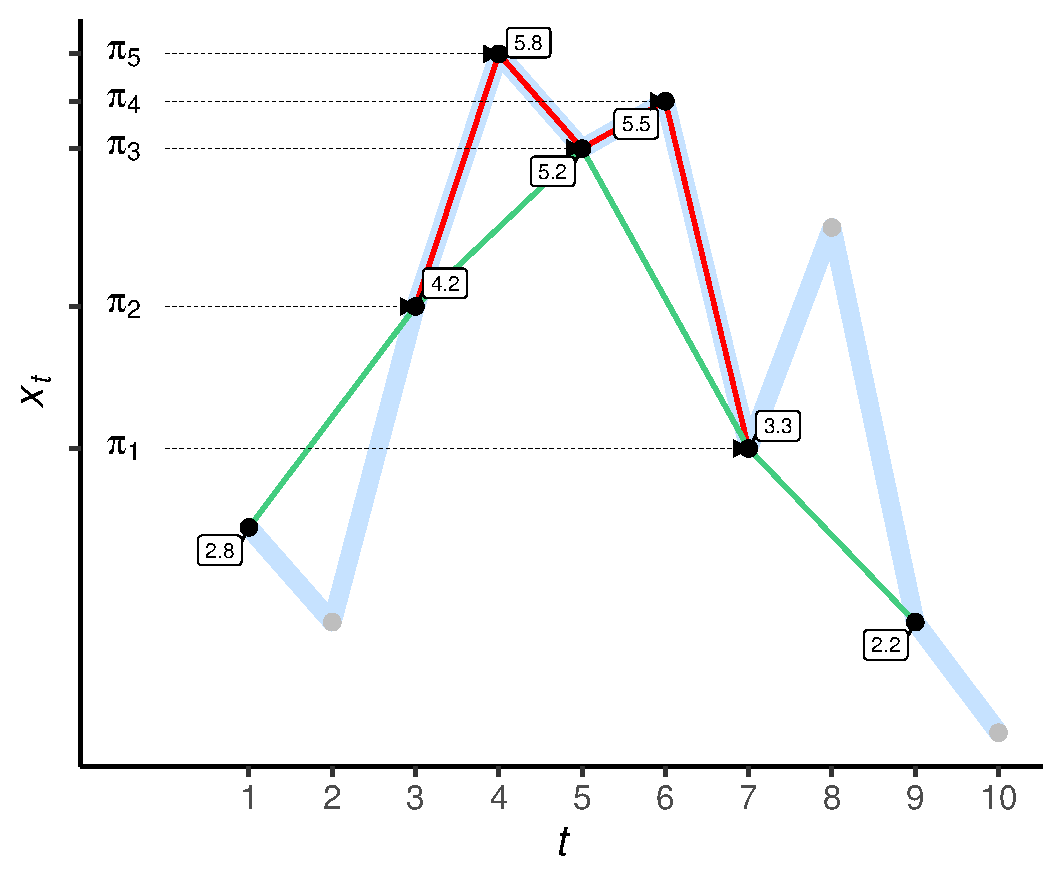
\includegraphics[width=.7\linewidth]{IntroBP}
	\caption{Illustration of the Bandt and Pompe coding}
	\label{Fig:IntroBP}
\end{figure}

After computing all the symbols, one obtains the histogram of proportions $\bm h = (h(j))_{1\leq j\leq D!}$.
Such histogram estimates the (unknown, in general) probability distribution function of these patterns.
The next step into the characterization of the time series is computing descriptors from this histogram.

The first descriptor is a measure of the disorder of the system.
The most frequently used feature for this is the Normalized Shannon entropy, defined as
\begin{equation}
	H(\bm h) = -\frac{1}{\log D!} \sum_{j=1}^{D!} h(j) \log h(j),
\end{equation}
with the convention that terms in the summation for which $h(j)=0$ are null.
This quantity is bounded in the unit interval. 
It is zero when $h(j)=1$ for some $j$ (and, thus, all other bins are zero), and one when $h(j)=1/D!$ for every $j$ (the uniform probability function).

Although very expressive, the Normalized Shannon Entropy is not able to describe all possible underlying dynamics.
In particular, for intermediate values of $H$, there is a wide variety of situations worth characterizing.
To this aim, \citet{LopezRuiz1995} proposed using the disequilibrium  $Q$, a measure of how far $\bm h$ is from an equilibrium or noninformative distribution.
They employed the Euclidean distance between $\bm h$ and the uniform probability function.

The Jensen-Shannon distance between $\bm h$ and the probability function $\bm u=(u(1), u(2), \dots, u(D!))$ stems as a more adequate measure of such a distance:
\begin{equation}
	Q'(\bm{h}, \bm{u}) = \sum_{\ell=1}^{D!} \Big(h(\ell) \log\frac{h(\ell)}{u(\ell)} +
	u(\ell) \log\frac{u(\ell)}{h(\ell)}
	\Big).
	\label{eq:JensenShannon}
\end{equation}
This has been the preferred distance function since its proposal by \citet{Lamberti2004}.
Most works consider the uniform distribution $\bm u = (1/D!, 1/D!, \dots, 1/D!)$ as the reference model.

The quantity~\eqref{eq:JensenShannon} is also called ``disequilibrium.''
The normalized disequilibrium is $ Q=Q'/\max\{Q'\}$, and we chose to work with the uniform probability distribution function as the equilibrium law.
Under these conditions holds that
$$
\max\{Q'\} = -2\Big[
\frac{D!+1}{D!} \log(D!+1) - 2 \log(2D!) + \log D!
\Big].
$$

With this, \citet{Lamberti2004} proposed $C=HQ$ as a measure of the Statistical Complexity of the underlying dynamics.
Notice that both $H$ and $Q$ are normalized quantities, so also is $C$. 
Moreover, $C$ is capable of discerning between different degrees of periodicity, among other relevant properties.

A time series can then be mapped into a point in the $H\times C$ plane.

\subsection{The Entropy-Complexity Plane}\label{Sec:HCPlane}

The Entropy-Complexity plane is the set of all possible points $(h,c)$ that can be produced by arbitrary time series analyzed with embedding dimension $D$ that are mapped on histograms of $D!$ bins.
The time delay is irrelevant, and we consider infinitely long series.

Let us consider two extreme cases:
\begin{enumerate}[label=Case~\Roman*., align=left, leftmargin=*]
	\item 	Strictly monotonically increasing or decreasing series produce a single pattern, so the other $D!-1$ bins of the histogram are zero. 
	The entropy is zero, and the distance to the uniform distribution is maximal. 
	Therefore, the complexity is zero, and such series are mapped onto the point $(0,0)$.
	\item 	White noise produces a histogram of equal proportions $1/D!$ and maximal entropy. 
	The distance to the equilibrium distribution is zero. 
	Thus, such series are mapped onto the point $(1,0)$.
\end{enumerate}

\citet{SomeFeaturesoftheLMCStatisticalComplexity} proved that, for a fixed value of entropy, there are two extreme values of complexity.
\citet{martin2006generalized}, using geometrical arguments on the space of configurations, found expressions for such boundaries.
The lower boundary $C_{\min}$ is smooth, while the upper $C_{\max}$ is defined by $D!-1$ pieces.
The upper boundary converges to a smooth curve when $D\to\infty$.


Fig.~\ref{fig:Boundaries} shows the boundaries of the $H\times C$ plane for the embedding dimensions $D=3$ (red) $D=4$ (green), and $D=5$ (blue).
The inset plot highlights the fine structure of the upper boundary inside the rectangle.
The jagged structure of $C_{\max}$ increases the difficulty of finding distributions for the points in the $H\times C$ plane.

\begin{figure}[hbt]
	\centering
	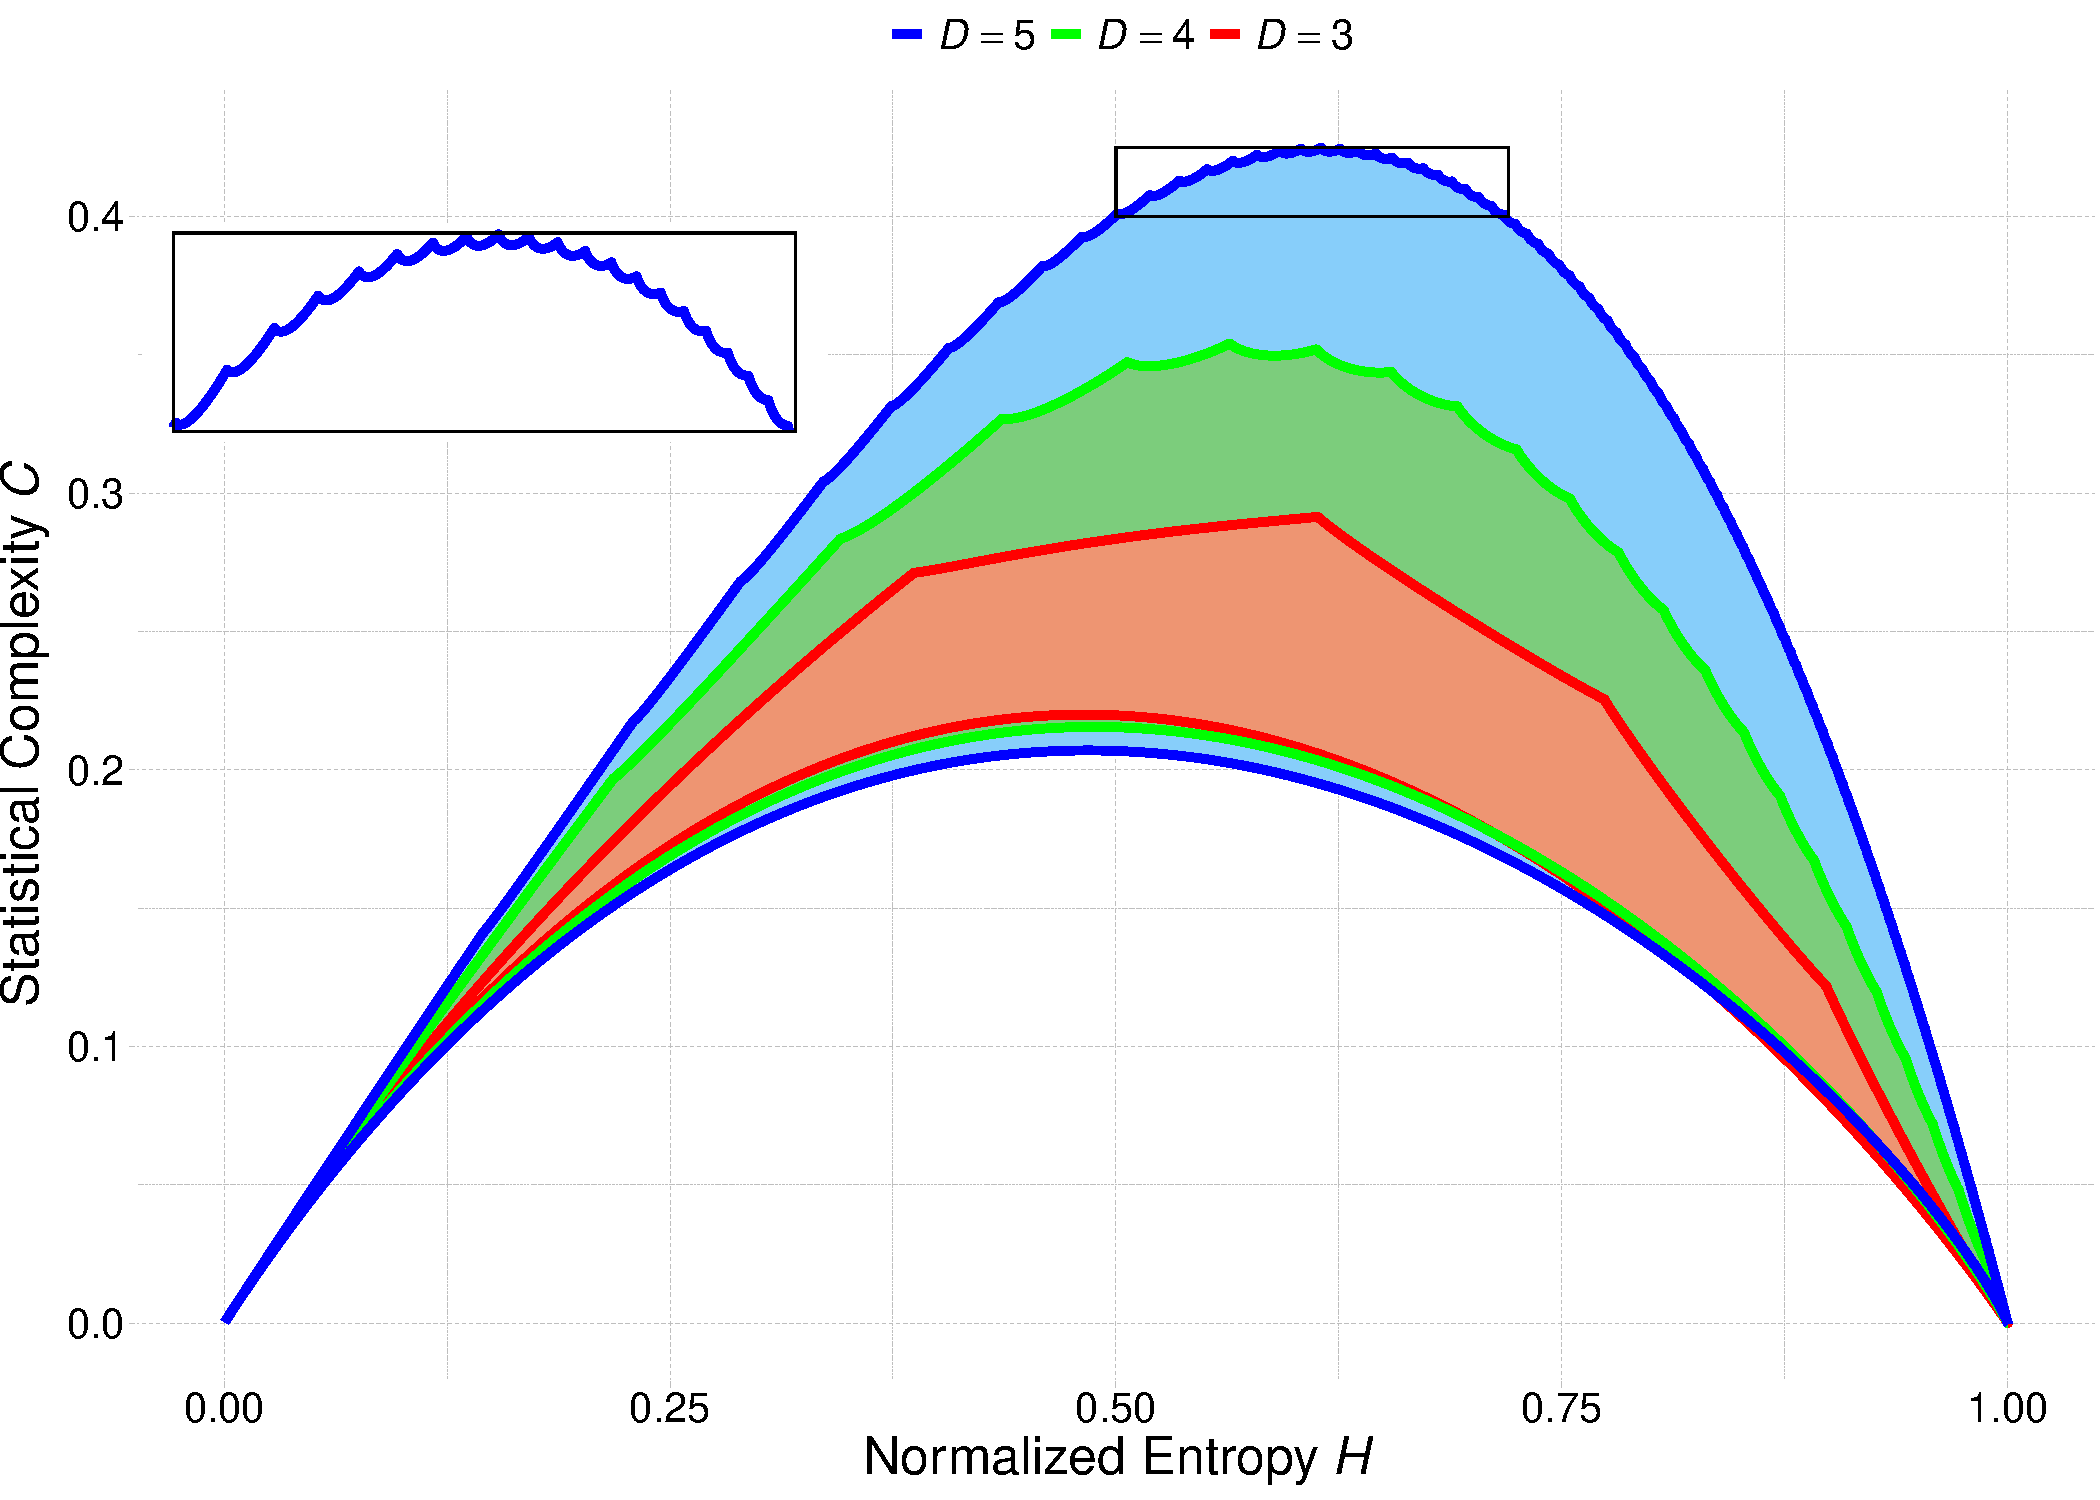
\includegraphics[width=.7\linewidth]{Figures/BoundariesPlot}
	\caption{Boundaries of the $H\times C$ plane for dimension embeddings $D=3,4,5$.}\label{fig:Boundaries}
\end{figure}

We illustrate the use of the Entropy-Complexity plane ($H\times C$) with the following time series:
\begin{itemize}
	\item Colored $k$-noise, or $f^{-k}$ noise: white ($k=0$), $k=1/2$, pink ($k=1$), $k=3/2$, red ($k=2$), $k=5/2$, and $k=3$;
	\item Chaotic logistic series $x_t = r x_{t-1} (1 - x_{t-1})$, with $r=3.6$ and $4$;
	\item Deterministic series: monotonic increasing ($\log(x_t+0.1)$, $x_t=\{1,2,\dots,10^4$) and periodic ($\sin(2x_t)\cos(2x_t)$, with $0\leq x_t\leq 2\pi$ over ten thousand equally spaced points).
\end{itemize}
In all cases, we used $D=6$ and $\tau=1$.
Fig.~\ref{fig:Histograms} shows nine of the histograms produced by these series using the Mersenne-Twister pseudorandom number generator;
we omitted those corresponding to the deterministic series, as they produce one and two nonzero bins.

\begin{figure}[hbt]
	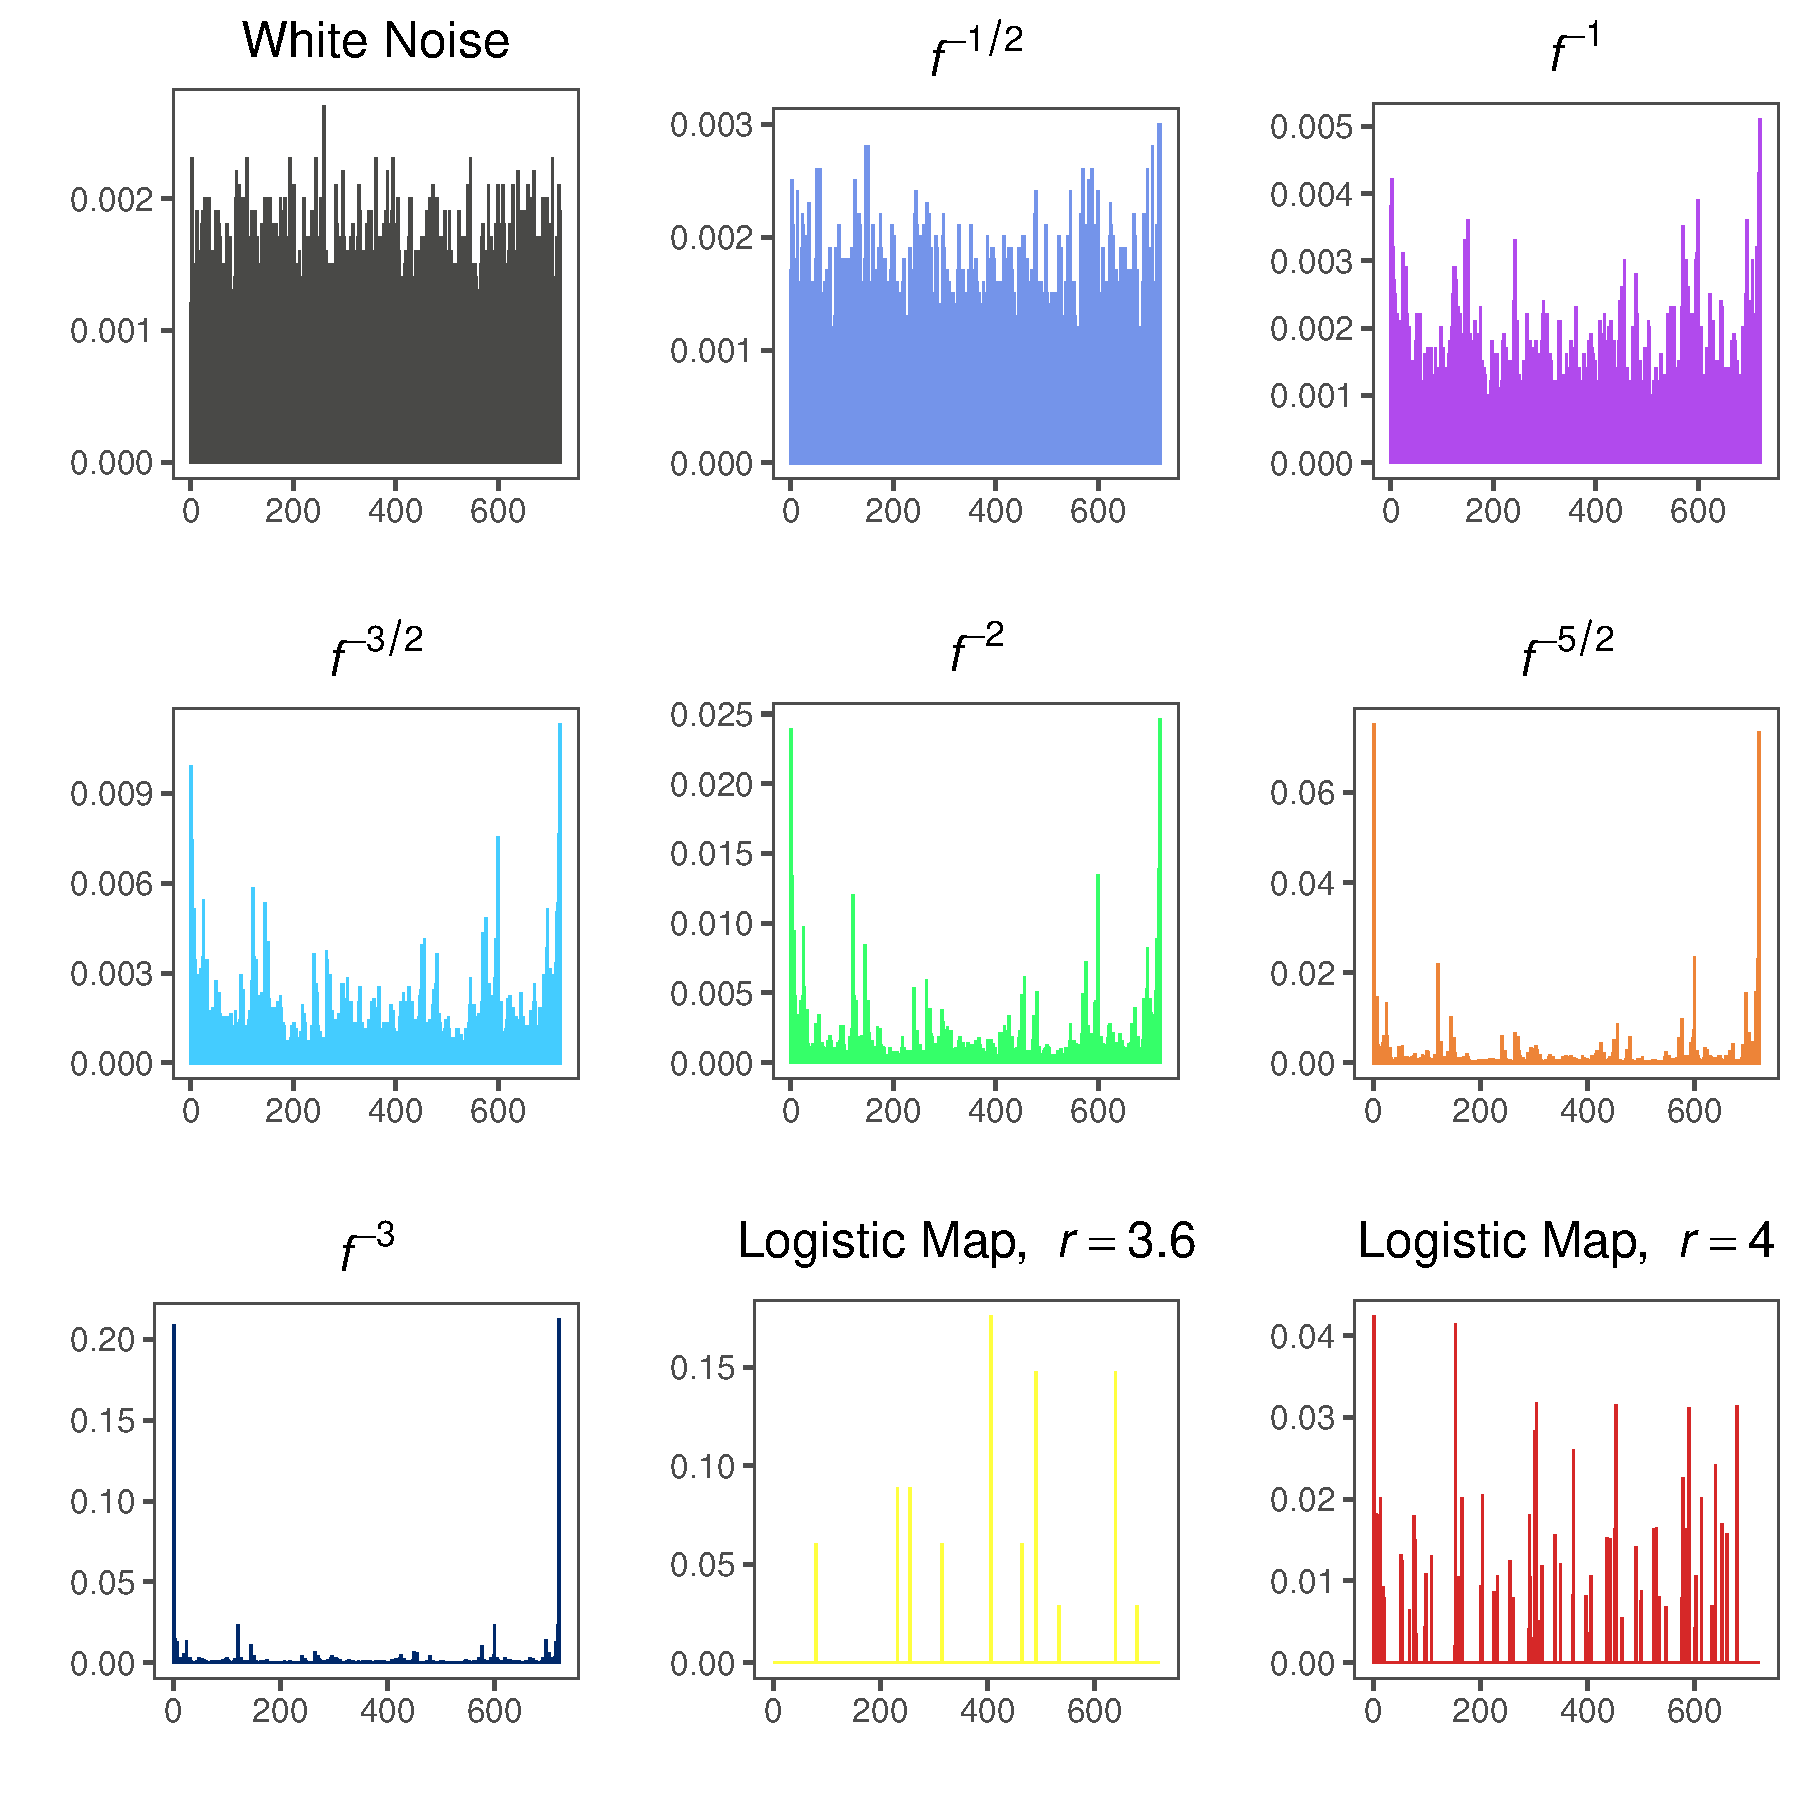
\includegraphics[width=\linewidth]{Figures/h.pdf}
	\caption{Patterns histograms of selected time series  for dimension embedding $D = 6$, time delay $\tau = 1$, and sequence length $T = \num[scientific-notation=true]{e4}$.}
	\label{fig:Histograms}
\end{figure}

Fig.~\ref{fig:AllSystems} shows the $H\times C$ plane with the bounds for $D=6$, the time series, and the points they were mapped onto.
The points due to $f^{-k}$ noises appear joined by dotted segments.
It is noticeable that deterministic patterns have more complexity than random ones.
Also, points related to $f^{-k}$ noises tend to clutter for $k<1$, having the highest entropy values, as can be seen in Fig.~\ref{fig:RightMostCorner}.

\begin{figure}[hbt]
	\centering
	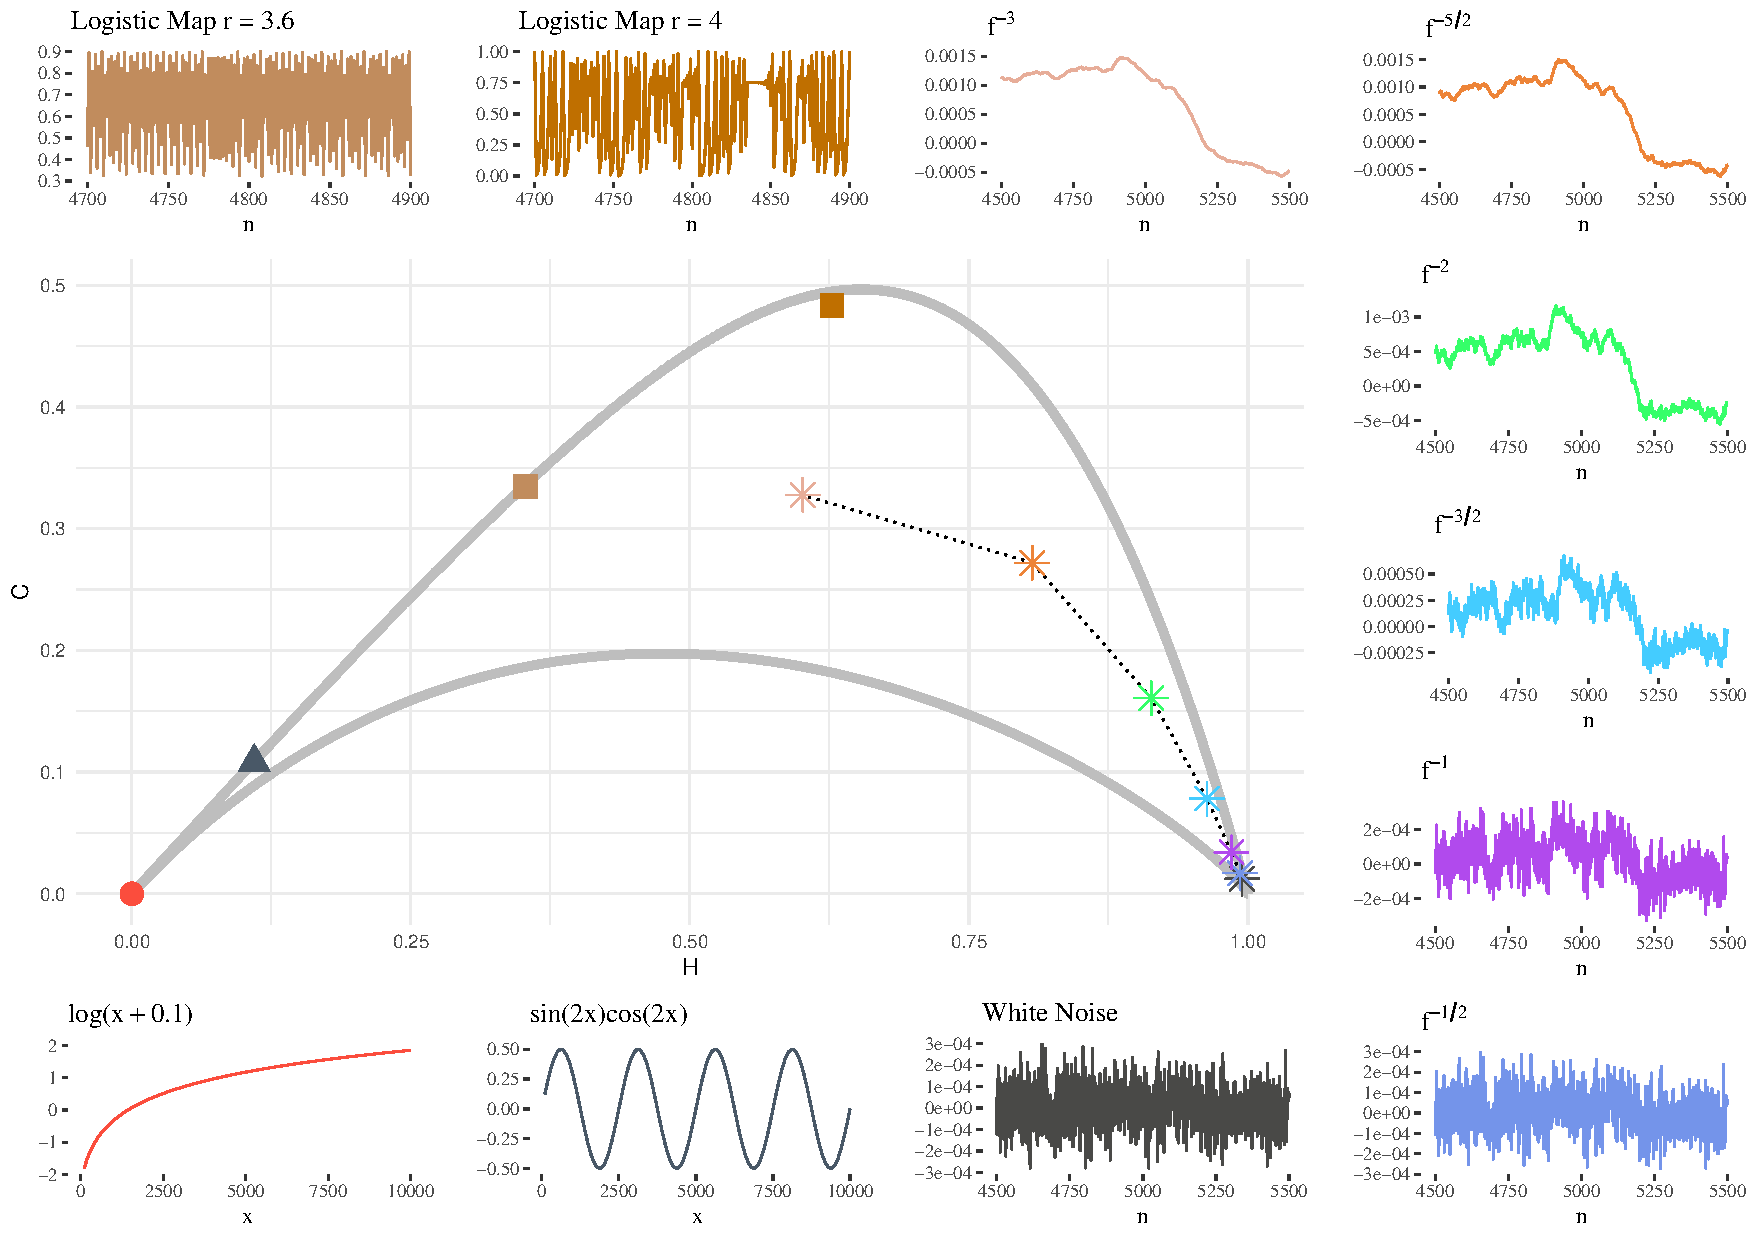
\includegraphics[width=\linewidth]{AllSystems}
	\caption{Eleven systems and their points in the $H\times C$ plane for dimension embedding $D = 6$, time delay $\tau = 1$, and sequence length $T = \num[scientific-notation=true]{e4}$.}
	\label{fig:AllSystems}
\end{figure}

Fig.~\ref{fig:RightMostCorner} shows the rightmost lower corner of the $H\times C$ plane, emphasizing the location of the white ($k=0$), $k=1/2$, and pink ($k=1$) noises.
In particular, notice that the point associated to white noise is not at $(1,0)$, as consequence of being obtained from a finite rather than infinite length sequence.

\begin{figure}[hbt]
	\centering
	\includegraphics[width=\linewidth]{RightMostCorner}
	\caption{Representations of white noise, $f^{-1/2}$, and $f^{-1}$ noise in the $H \times C$ plane  for dimension embedding $D = 6$, time delay $\tau = 1$, and sequence length $T = \num[scientific-notation=true]{e4}$.}
	\label{fig:RightMostCorner}
\end{figure}

Due to the infinitude of white noise sequences, although these sequences have the characteristic of presenting high values of entropy and low statistical complexity, their points will not necessarily be located in $(1, 0)$, but in a surrounding region.
Our study's focus is to assess pure randomness by analyzing the empirical distribution of the points produced by true random sequences of finite size and obtaining regions of confidence in the $H \times C$ plane.

\subsection{The Entropy-Complexity Plane in the Literature}\label{Sec:BPApplications}

Initial works on the characterization of white noises with permutation entropy arose from the need to discriminate between them and chaotic maps \citep{rosso2013characterization, xiong2020complexity}.
Notice that the logistic map has been used for pseudorandom number generation; cf. \citet{AnalyzingLogisticMapPseudorandomNumberGeneratorsforPeriodicityInducedbyFinitePrecisionFloatingPointRepresentation} and the references therein.
It was found that measures of statistical complexity were able to efficiently quantify the performance of pseudorandom number generators, expanding the possibilities of using Information Theory descriptors with the Bandt-Pompe symbolization \citep{larrondo2013statistical, gonzalez2005statistical}.

Table~\ref{Tab:Literature} presents a summary of the main works in the literature that perform analysis of non-chaotic algorithmic generators, according to their features in the $H\times C$ plane.
We also provide the length $T$ and embedding dimension $D$ of the time series under scrutiny.
The following algorithmic generators were analyzed:
\begin{itemize}
	\item Mother RNG, available in Marsaglia's website \citep[MOT,][]{marsaglia1994yet};
	\item Multiple with carry RNG \citep[MWC,][]{marsaglia1994yet};
	\item Combo RNG \citep[COM,][]{marsaglia1994yet};
	\item Lehmer RNG \citep[LEH,][]{payne1969coding};
	\item Fractional Brownian motion (fBm) and fractional Gaussian noise (fGn); see \citet{bardet2003generators};
	\item Colored noise with power spectrum $f^{-k}$ with $k \geq 0$~\citep{larrondo2012matlab};
	\item Linear Congruential Generator \citep[LCG,][]{knuth1997sorting}.
\end{itemize}


\begin{table}[hbt]
	\caption{Results of the main works of white noise sequences analysis in the $H \times C$ plane.}
	\label{Tab:Literature}
	\centering
	\begin{tabular}{llcccc b{5.4em}}
		\toprule
		Reference & PRNG & $T$ & $D$ & $H$ & $C$ & Considered random? \\ 
		\midrule
		\citeauthor{larrondo2013statistical} (\citeyear{larrondo2013statistical}) &  MOT & NA & 6 & $\cong 0.9969$ & $\cong 0$ & no\\
		\cmidrule(lr){1-7}
		\citeauthor{gonzalez2005statistical} (\citeyear{gonzalez2005statistical})  &  MWC & 65536 & NA & $\cong 1$ & $0.3$ & yes \\
		&  MOT & 65536 & NA & $\cong 1$ & $0.3$ & yes \\
		&  COM & 65536 & NA & $\cong 1$ & $0.05$ & yes\\
		\cmidrule(lr){1-7}
		\citeauthor{RandomNumberGeneratorsCausality} (\citeyear{RandomNumberGeneratorsCausality}) &  LEH & \num[scientific-notation=true]{5 e6} & 5 & $\cong 1$ & $10^{-4}$ & yes \\
		&  MOT & \num[scientific-notation=true]{5 e6} & 5 & $\cong 1$ & $10^{-4}$ & yes\\
		&  MWC & \num[scientific-notation=true]{5 e6} & 5 & $\cong 1$ & $10^{-4}$ & yes\\
		\cmidrule(lr){1-7}
		\citeauthor{rosso2013characterization} (\citeyear{rosso2013characterization}) &  LCG & \num[scientific-notation=true]{1 e7} & 6 & $0.997871$ & $0.005101$ & no\\
		\cmidrule(lr){1-7}
		\citeauthor{xiong2020complexity} (\citeyear{xiong2020complexity}) &  fGn & \num[scientific-notation=true]{2 e17} & 6 & $\cong 1$ & $\cong 0$ & yes \\
		& $f^{-k}$ & \num[scientific-notation=true]{2 e17} & 6 & $\cong 1$ & $\cong 0$ & yes \\
		\bottomrule
	\end{tabular}
\end{table}

None of these works provide $p$-values or hypothesis tests for their analysis.
The focus of the articles is finding the set of descriptors that best discriminates chaos from noise.
The authors make assessments about the randomness of sequence on ad hoc visual inspection of the point's location in the $H\times C$ plane.
Our work fills such a gap for finite sequences of white noise and proposes a methodology that can be extended to any other situation.

\section{Proposed Method}\label{Sec:Proposal}

In this section, we formalize the task of building confidence regions in the Entropy-Complexity manifold.
Then, we present our proposal to change space through the algorithm of the principal components analysis.
Our goal is to find a latent space representative of the data without the restrictions of the $H\times C$ plane's boundaries.
Through this new representation of the data, we calculate empirical regions with different levels of confidence.
Finally, after calculating these regions, we build a test statistic that determines the probability that a given sequence belongs to the distribution of the points provided.

\subsection{Overall Framework}\label{Sec:OverallFramework}

Our methodology consists of the following steps:
\begin{enumerate}
	\item\label{item:Methodology1} Observe a large number of true random white noise sequences (TRWNS).
	\item\label{item:Methodology2} Map each TRWNS onto a point in the $H\times C$ plane.
	\item\label{item:Methodology3} Obtain the principal components of these points.
	\item\label{item:Methodology4} Compute enclosing boxes in the principal components space.
	\item\label{item:Methodology5} Transform the coordinates of these boxes back to the $H\times C$ plane.
\end{enumerate}

\subsection{True Random Numbers}\label{Sec:TRNG}

Random numbers are used in many fields, from gambling to cryptography, to guarantee a secure, realistic, or unpredictable behavior. 
Pseudorandom results can be achieved by software in a deterministic way, but some applications need actual random numbers (despite the somewhat elusive nature of actual randomness).
Randomness can be observed in unpredictable real-world phenomena like cathodic radiation or atmospheric noise.
%In this study we used two sources of real random numbers. 
%The first is based on vacuum states to generate random quantum numbers described by \citeauthor{RNGVacuumStates}~(\citeyear{RNGVacuumStates}), the second one is based on atmospheric noise captured by a cheap radio receiver presented at \url{www.random.org}.

In this study, we used two sources of true random numbers, both from the observation and measurement of physical phenomena.
The first uses vacuum states. 
The setup consists of an ordinary laser source to generate a local oscillator (LO), a half-wave plate, a polarizing beamsplitter (BPS), and two balanced detectors working together adding or subtracting the photocurrents results in a quadrature measurement of the LO or vacuum state. 
The distribution of the vacuum state is binned into $2^n$ equal parts (bins of the same size), assigning a fixed bit combination of length $n$ to each sample point in a given bin \citep{RNGVacuumStates}. 
The second one employs atmospheric noise captured by a cheap radio receiver with no filter for unwanted static sounds caused by atmospheric noise.
This generator was implemented over a distributed setup with radios located at different geographical locations sending random bits to a cloud server that processes data and hosts the values.
The history of this service and other information can be found at \citet{RandomOrg}.

We used \SI{54e6}{\byte} words from each physical generator, which approximately amounts \SI{200}{\mega\byte} of data.

%\textcolor{red}{Fornecer mais informações. Quantos dados em bits, ou bytes, ou outra unidade, foram empregados de cada fonte, e como foram armazenados. Precisão simples, certo?}

\subsection{Parameters Settings and Dataset}\label{Sec:Parameters}

We conducted an ablation study to identify the influence of the parameters $T$, $D$, and $\tau$ in the construction of empirical confidence regions.
We verified that the results involving the time delay parameter variation did not show significant differences in repeated experiments; therefore, in the sequel, we did no consider $\tau$ as a determining factor.
On the other hand, we found two relevant variables: 
the length of the sequence 
and the embedding dimension.
We, thus, employed the following factors:
\begin{itemize}
	\item Sequence length $T\in\mathcal T=\{ \num[scientific-notation=true]{e3}, \num[scientific-notation=true]{5 e4}\}$,
	\item Embedding dimension $D\in\mathcal D=\{3, 4, 5, 6\}$.
	%,and
	%\item Time delay $\tau=\{1, 10, 30, 50\}$.
\end{itemize}
and kept $\tau=1$, which is the most frequently used option.
The values of $D$ are within the range recommended in the literature~\citep{PermutationEntropyBandtPompe}.

Using this parametric space, we analyzed the different degrees of information captured by the ordinal patterns formed.
For the construction of the confidence regions presented, we used:
\begin{itemize}
	\item A set of \num{104596} points in the $H \times C$ plane, corresponding to sequences of length $T = 1000$, for each value of $D\in \mathcal D$, and
	\item  a set of \num{2093} points in the $H \times C$ plane, corresponding to sequences of length $T = 50000$, for each value of $D \in \mathcal D$.
\end{itemize}

We used the \texttt R platform \citep[][v.~4.0.3]{Rmanual} for data generation and analyses, and the \texttt{ggplot2} library \citep{ggplot2Wickman} for generating the plots.

\begin{comment}

\begin{figure}
\centering
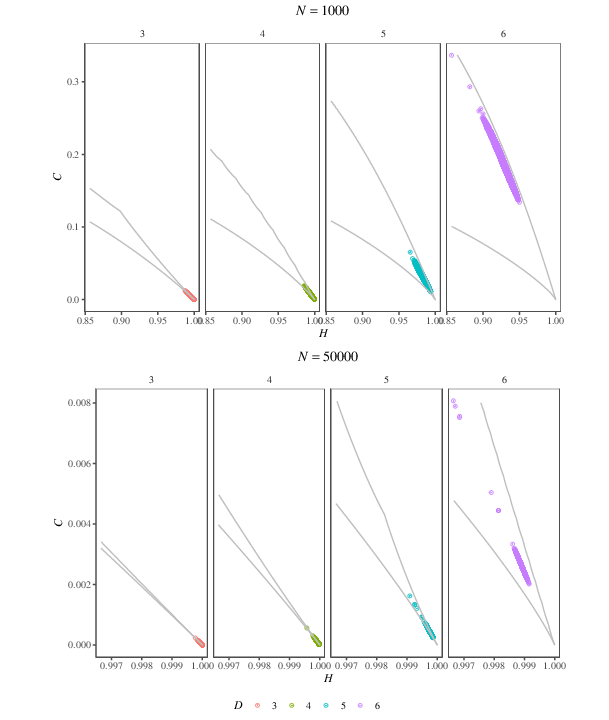
\includegraphics[width=\linewidth]{Figures/Points-PDF.png}
\caption{White noise samples considered during the construction of the proposed confidence regions.}
\label{fig:white-noise}
\end{figure}

\end{comment}

\subsection{Empirical Confidence Regions and $p$-values}\label{confidenceRegions}

%As we do not know the joint probability distribution of the pair $(h, c)$ for a sequence of random variables collectively independent and identically distributed according to a uniform law, studies involving classical bi-variate analysis, linear regression, and generalized linear models become unfeasible.

Our first approaches to analyzing sequences of points in the $H\times C$ plane produced by TRWNS verified that they, and usual transformations, are far from bivariate Gaussian and generalized Hyperbolic distributions \Mycite{MultivariateDistributionModelswithGeneralizedHyperbolicMargins}.
Different types of regression models of $C$ explained by $H$ did not produce acceptable results.
Thus, we adopted a non-parametric approach and made an empirical analysis of the data obtained from physical sources for using them as our reference in the search for confidence regions and $p$-values.
%Therefore, for the construction of our proposal, we adopted a non-parametric approach, making an empirical analysis of data obtained from physical sources and using them as our reference in the search for confidence regions.

%The set of all feasible pairs in the $H \times C$ plane is found in a compact subset of $\mathbbm{R}^2$, which has limits with explicit expressions for the boundaries of this closed manifold, dependent only on the dimension of the probability space considered, that is $D!$ in the traditional Bandt-Pompe method~\citep{martin2006generalized}.
%Due to such quotas, some limitations are generated, such as the absence of a representative distance metric and the difficulty of proposing confidence regions.
%In view of this, it is necessary to apply an orthogonal projection in the data for a new two-dimensional coordinate system to solve these restrictions.
%A classic proposal in these categories of problems is the principal component analysis algorithm~\citep{wold1987principal}.

Let $\utilde{x} =(x_1, x_2, \dots, x_N)$ be $N$ times series of length $T$, and define an embedding dimension $D$.
In the sequel, whenever possible, we will omit $T$ and $D$.
For each $n=1,2,\dots, N$, the time series $x_n$ is mapped onto the point $(h_n,c_n)$ in the $H\times C$ plane, thus $\utilde{hc}=\big((h_1,c_n), (h_2,c_2), \dots, (h_N,c_N)\big)$ are the points that correspond to the $N$ time series.
Fig.~\ref{fig:Methodology1} illustrates this step.
We will obtain confidence regions and $p$-values from $\utilde{hc}$.

The first step consists in finding and applying the principal components transformation to $\utilde{hc}$.
With this, we obtain the set of uncorrelated points $\utilde{uv}=\big((u_1,v_1), (u_2,v_2),\dots,(u_N,v_N)\big)$, in which $u_n$ and $v_n$ are the first and second principal components of $h_n$ and $v_n$, respectively.
This projection allows us to obtain a ``central'' point of the data set, around which we will build a rectangular box containing \SI{100}{\minusalphapercent} of the observations.
Such box is a variation of the bagplot \citep{TheBagplotaBivariateBoxplot}.
Notice that finding the smallest box that encloses $k$ out of $N$ points is difficult; cf.\ the work by \citet{SmallestKEnclosingRectangleRevisited}.

For simplicity, and without loss of generality, assume $N$ is odd.
\begin{enumerate}
	\item Find the indexes that sort the values of the first principal component $\bm u=(u_1,u_2,\dots,u_N)$ in ascending order: $\bm r=(r_1,r_2,\dots,r_N)$, i.e., $u_{r_1}$ is the minimum value, and $u_{r_N}$ is the maximum value.
	\item\label{item:Median} Find the point $(u,v)$ whose first principal component is the median: $(u_{r_{(N+1)/2}}, \cdot)$. Apply the inverse principal components transformation, and obtain $\bm P'=(h',v')$. Call the corresponding time series ``emblematic time series.''
	\item\label{item:Point1} Find the point $(u,v)$ whose first principal component is the quantile $\alpha/2$: $(u_{r_{[N\alpha/2]}}, \cdot)$.
	\item\label{item:Point2} Find the point $(u,v)$ whose first principal component is the quantile $1-\alpha/2$: $(u_{r_{[N(1-\alpha/2)]}}, \cdot)$.
	\item\label{item:Point3} The values $u_{r_{[N\alpha/2]}}$ and $u_{r_{[N(1-\alpha/2)]}}$ are the rightmost and leftmost bounds of the box, respectively.
	\item\label{item:Point4} The bottom bound of the box is the smallest second principal component value whose first principal component is at least $u_{r_{[N\alpha/2]}}$; denote this values $v_{\min}$.
	\item\label{item:Point5} The top bound of the box is the largest second principal value whose first principal component is at most $u_{r_{[N(1-\alpha/2)]}}$; denote this value $v_{\max}$.
	\item The corners of the box are 
	$(u_{r_{[N\alpha/2]}}, v_{\min})$, 
	$(u_{r_{[N\alpha/2]}}, v_{\max})$, 
	$(u_{r_{[N(1-\alpha/2)]}}, v_{\min})$ and 
	$(u_{r_{[N(1-\alpha/2)]}},v_{\max})$.
	\item\label{item:BoxHxC} Apply the inverse principal components transformation to these corners obtaining $\bm P_1=(h_{v_1}, c_{v_1})$, $\bm P_2=(h_{v_2},h_{v_2})$, $\bm P_3=(h_{v_3}, c_{v_3})$ and $\bm P_4=(h_{v_4},c_{v_4})$.
\end{enumerate}

Fig.~\ref{fig:methodology} illustrates these steps.
%
Fig.~\ref{fig:Methodology1} shows the points produced by TRWNS in the $H\times C$ plane.
The blue box includes a certain percentage of points, with sides parallel to the $H$ and $C$ axes.
The area in the $H\times C$ plane overestimates the desired proportion and may include ``unacceptable'' points.
%
Fig.~\ref{fig:Methodology2} shows the previous points projected onto the principal components space (steps~\ref{item:Median} to~\ref{item:Point5}).
The red box includes the same percentage of desired points, with axes parallel to the first and second principal components.
We highlighted in red the point whose first principal component is the median of the observed values.
%
Fig.~\ref{fig:Methodology3} shows the result of projecting back the red box from the principal components space to the $H\times C$ plane (step~\ref{item:BoxHxC}).
The comparison of the red and blue boxes shows that the area has been reduced, thus improving the test's power.

\begin{figure}[hbt]
	\centering
	%    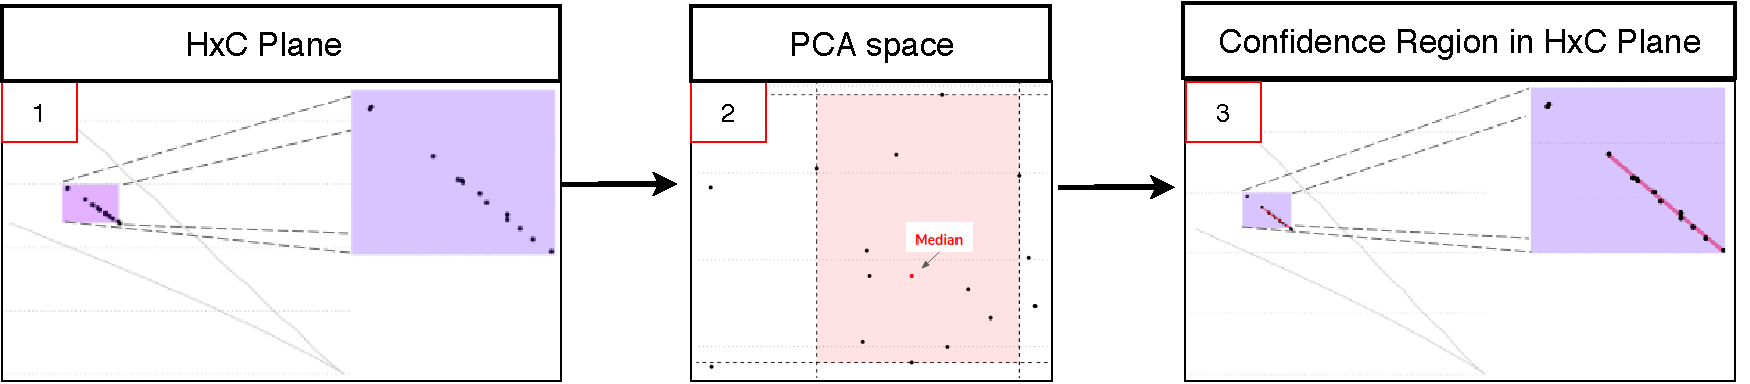
\includegraphics[width=\linewidth]{Figures/Methodology.pdf}
	\subfloat[Mapping true white noise random sequences onto the $H\times C$ plane.\label{fig:Methodology1}]{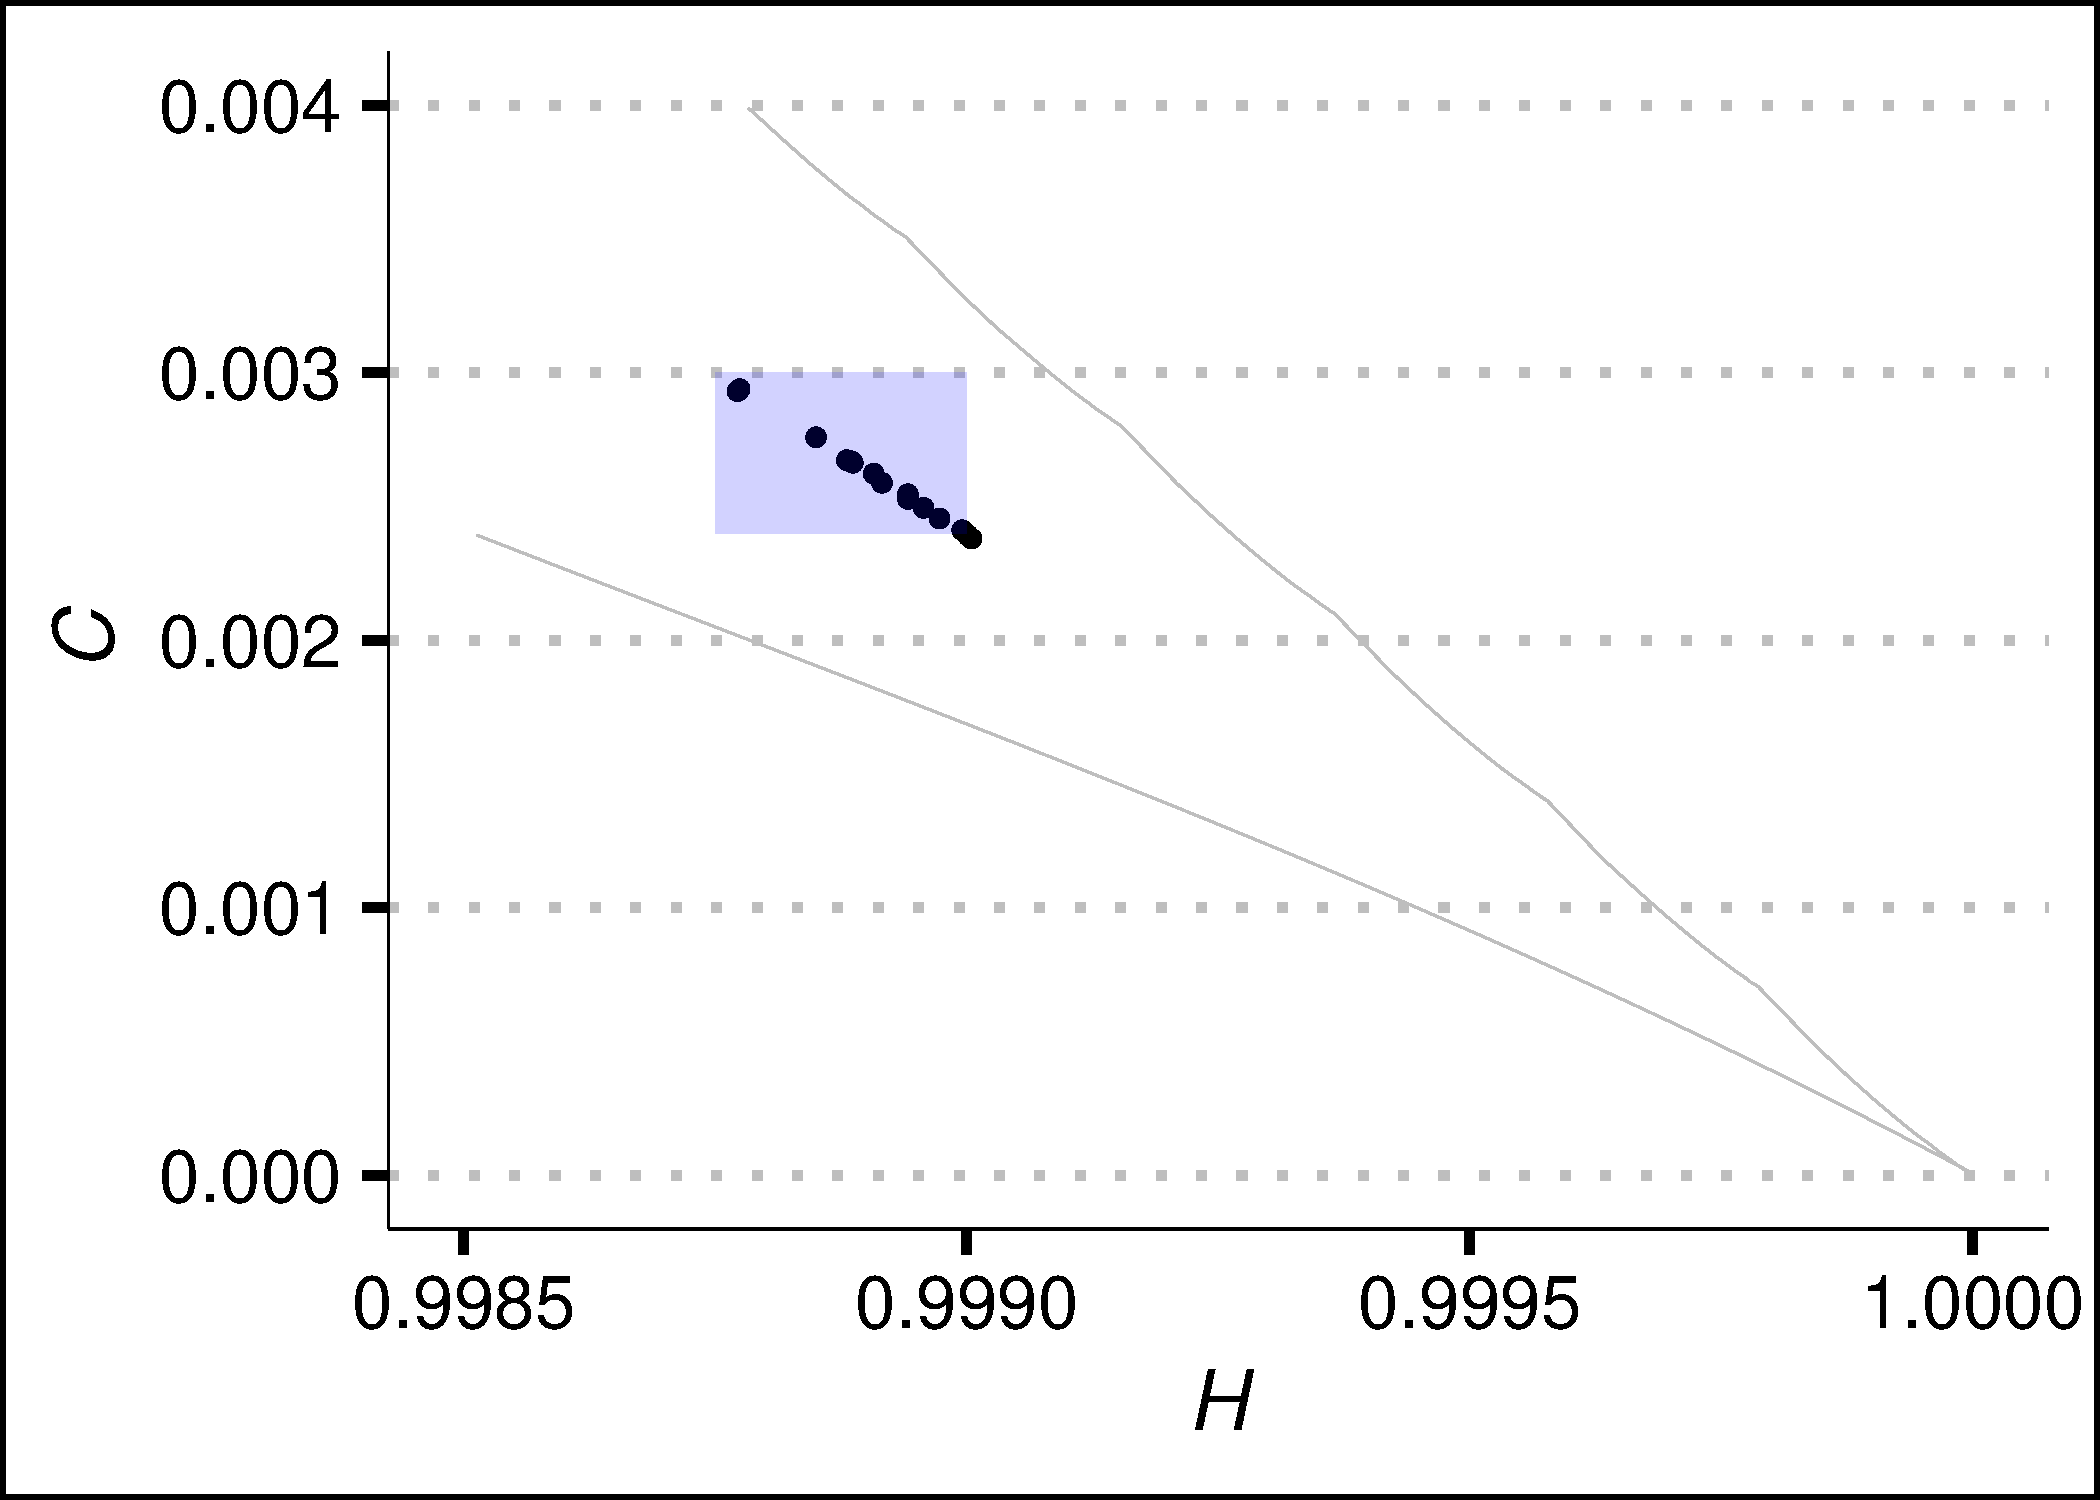
\includegraphics[width=.33\linewidth]{step1}}
	\subfloat[Transformation of the points in the $H\times C$ plane by Principal Components, and determination of minimal boxes.\label{fig:Methodology2}]{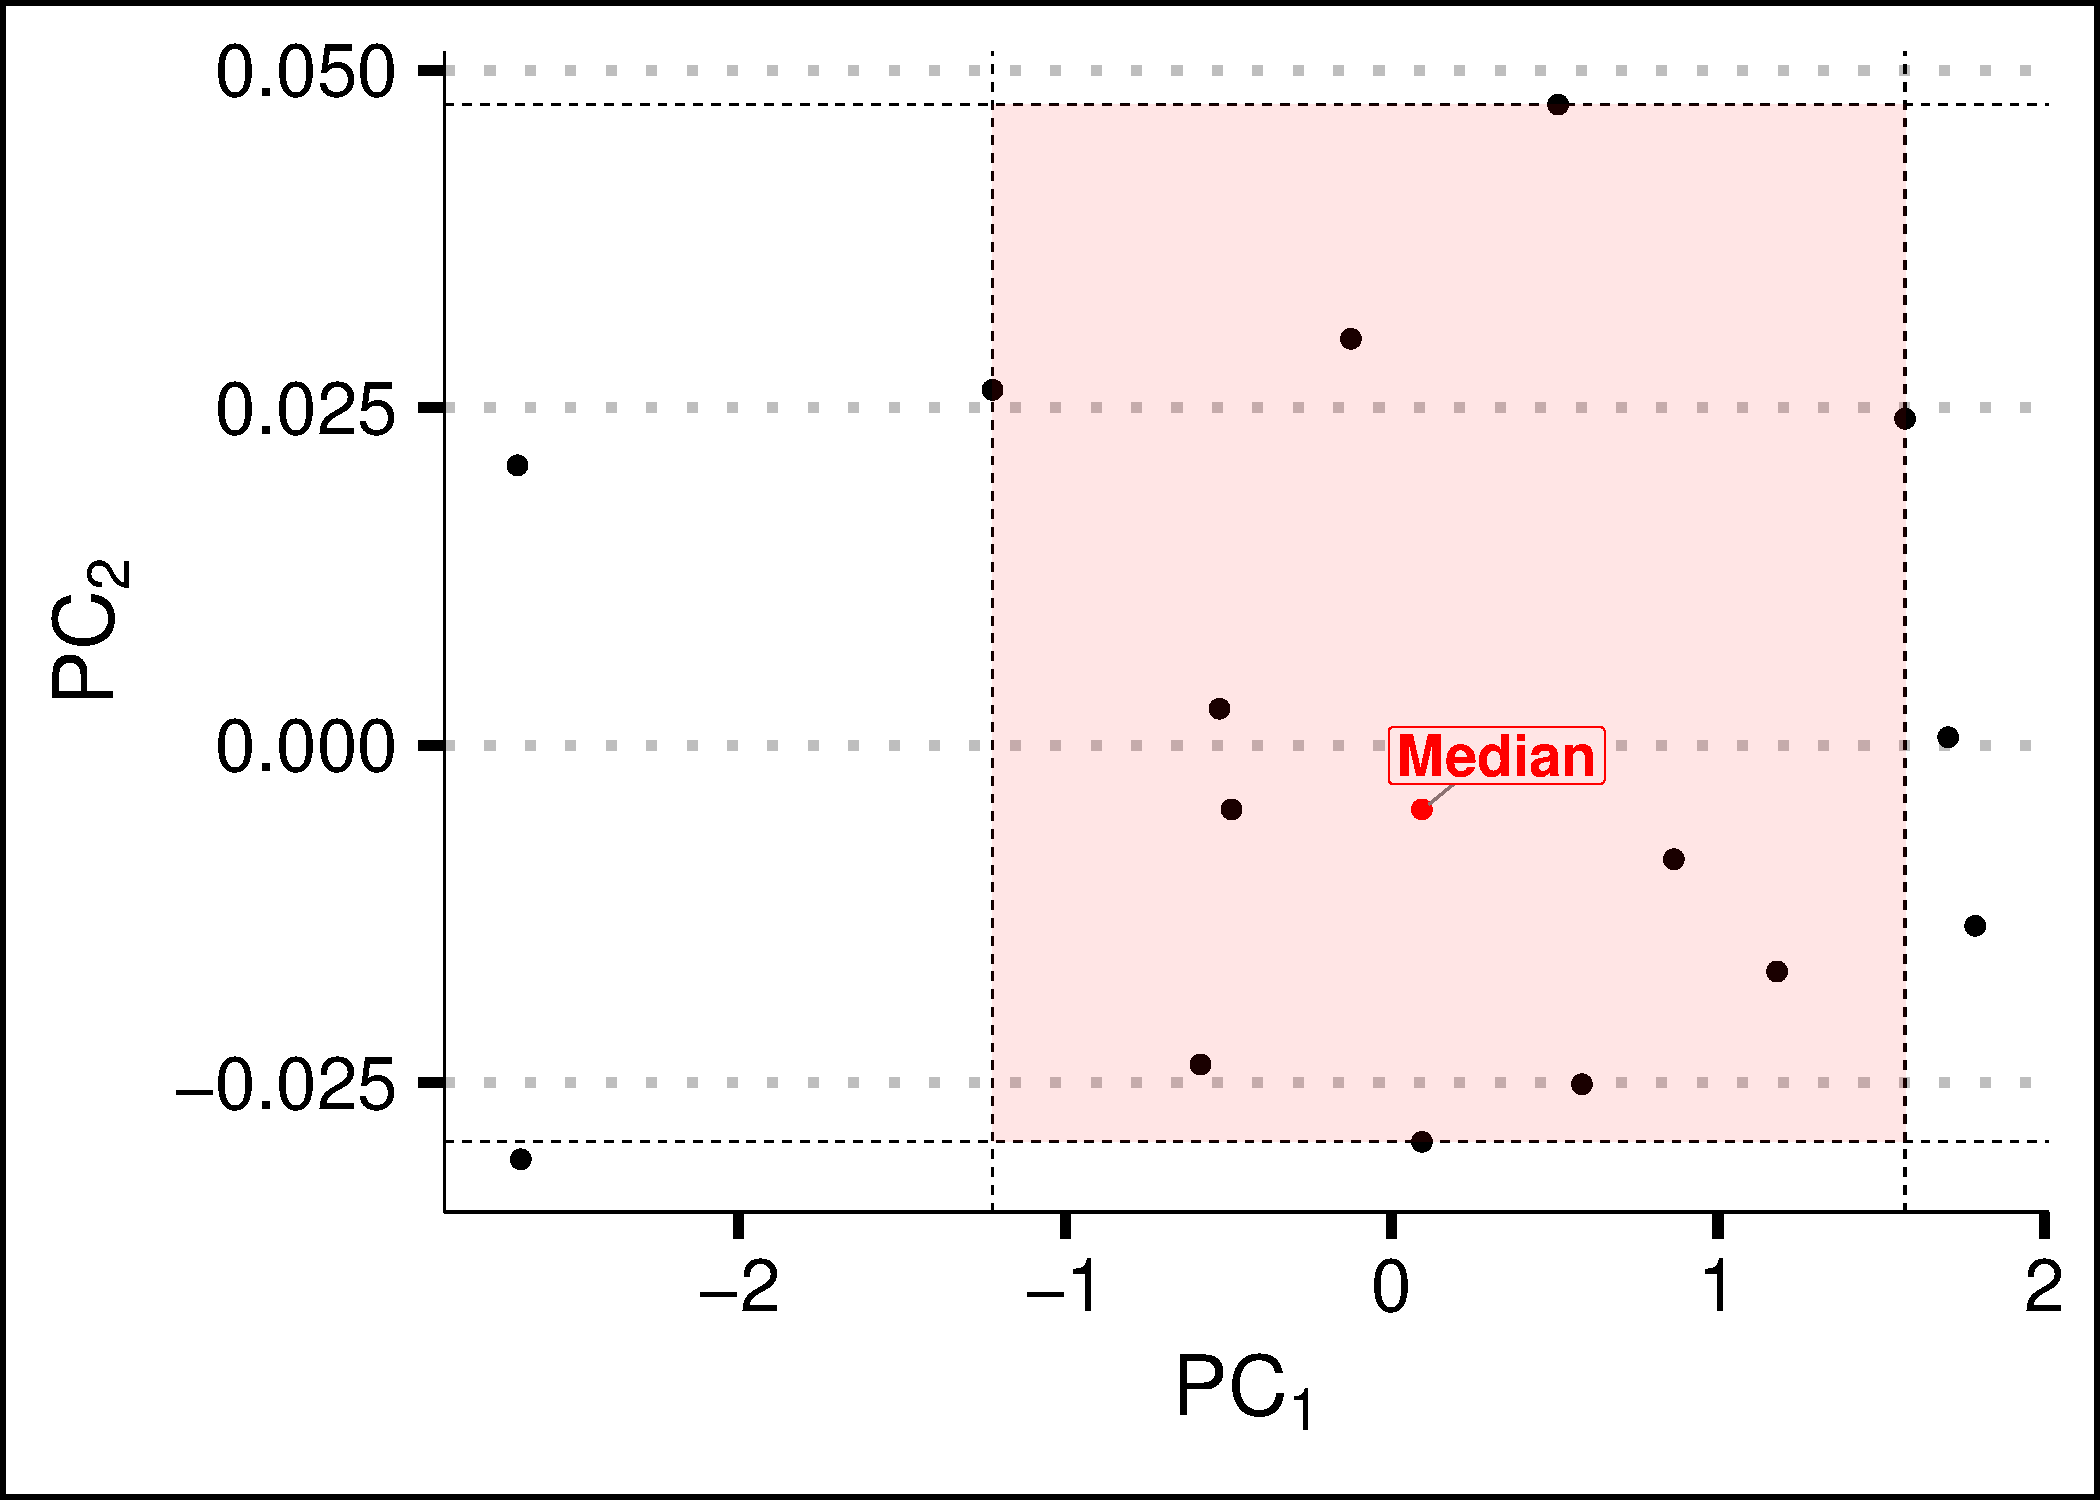
\includegraphics[width=.33\linewidth]{step2}}
	\subfloat[Inverse transformation from the Principal Components plane to the $H\times C$ plane.\label{fig:Methodology3}]{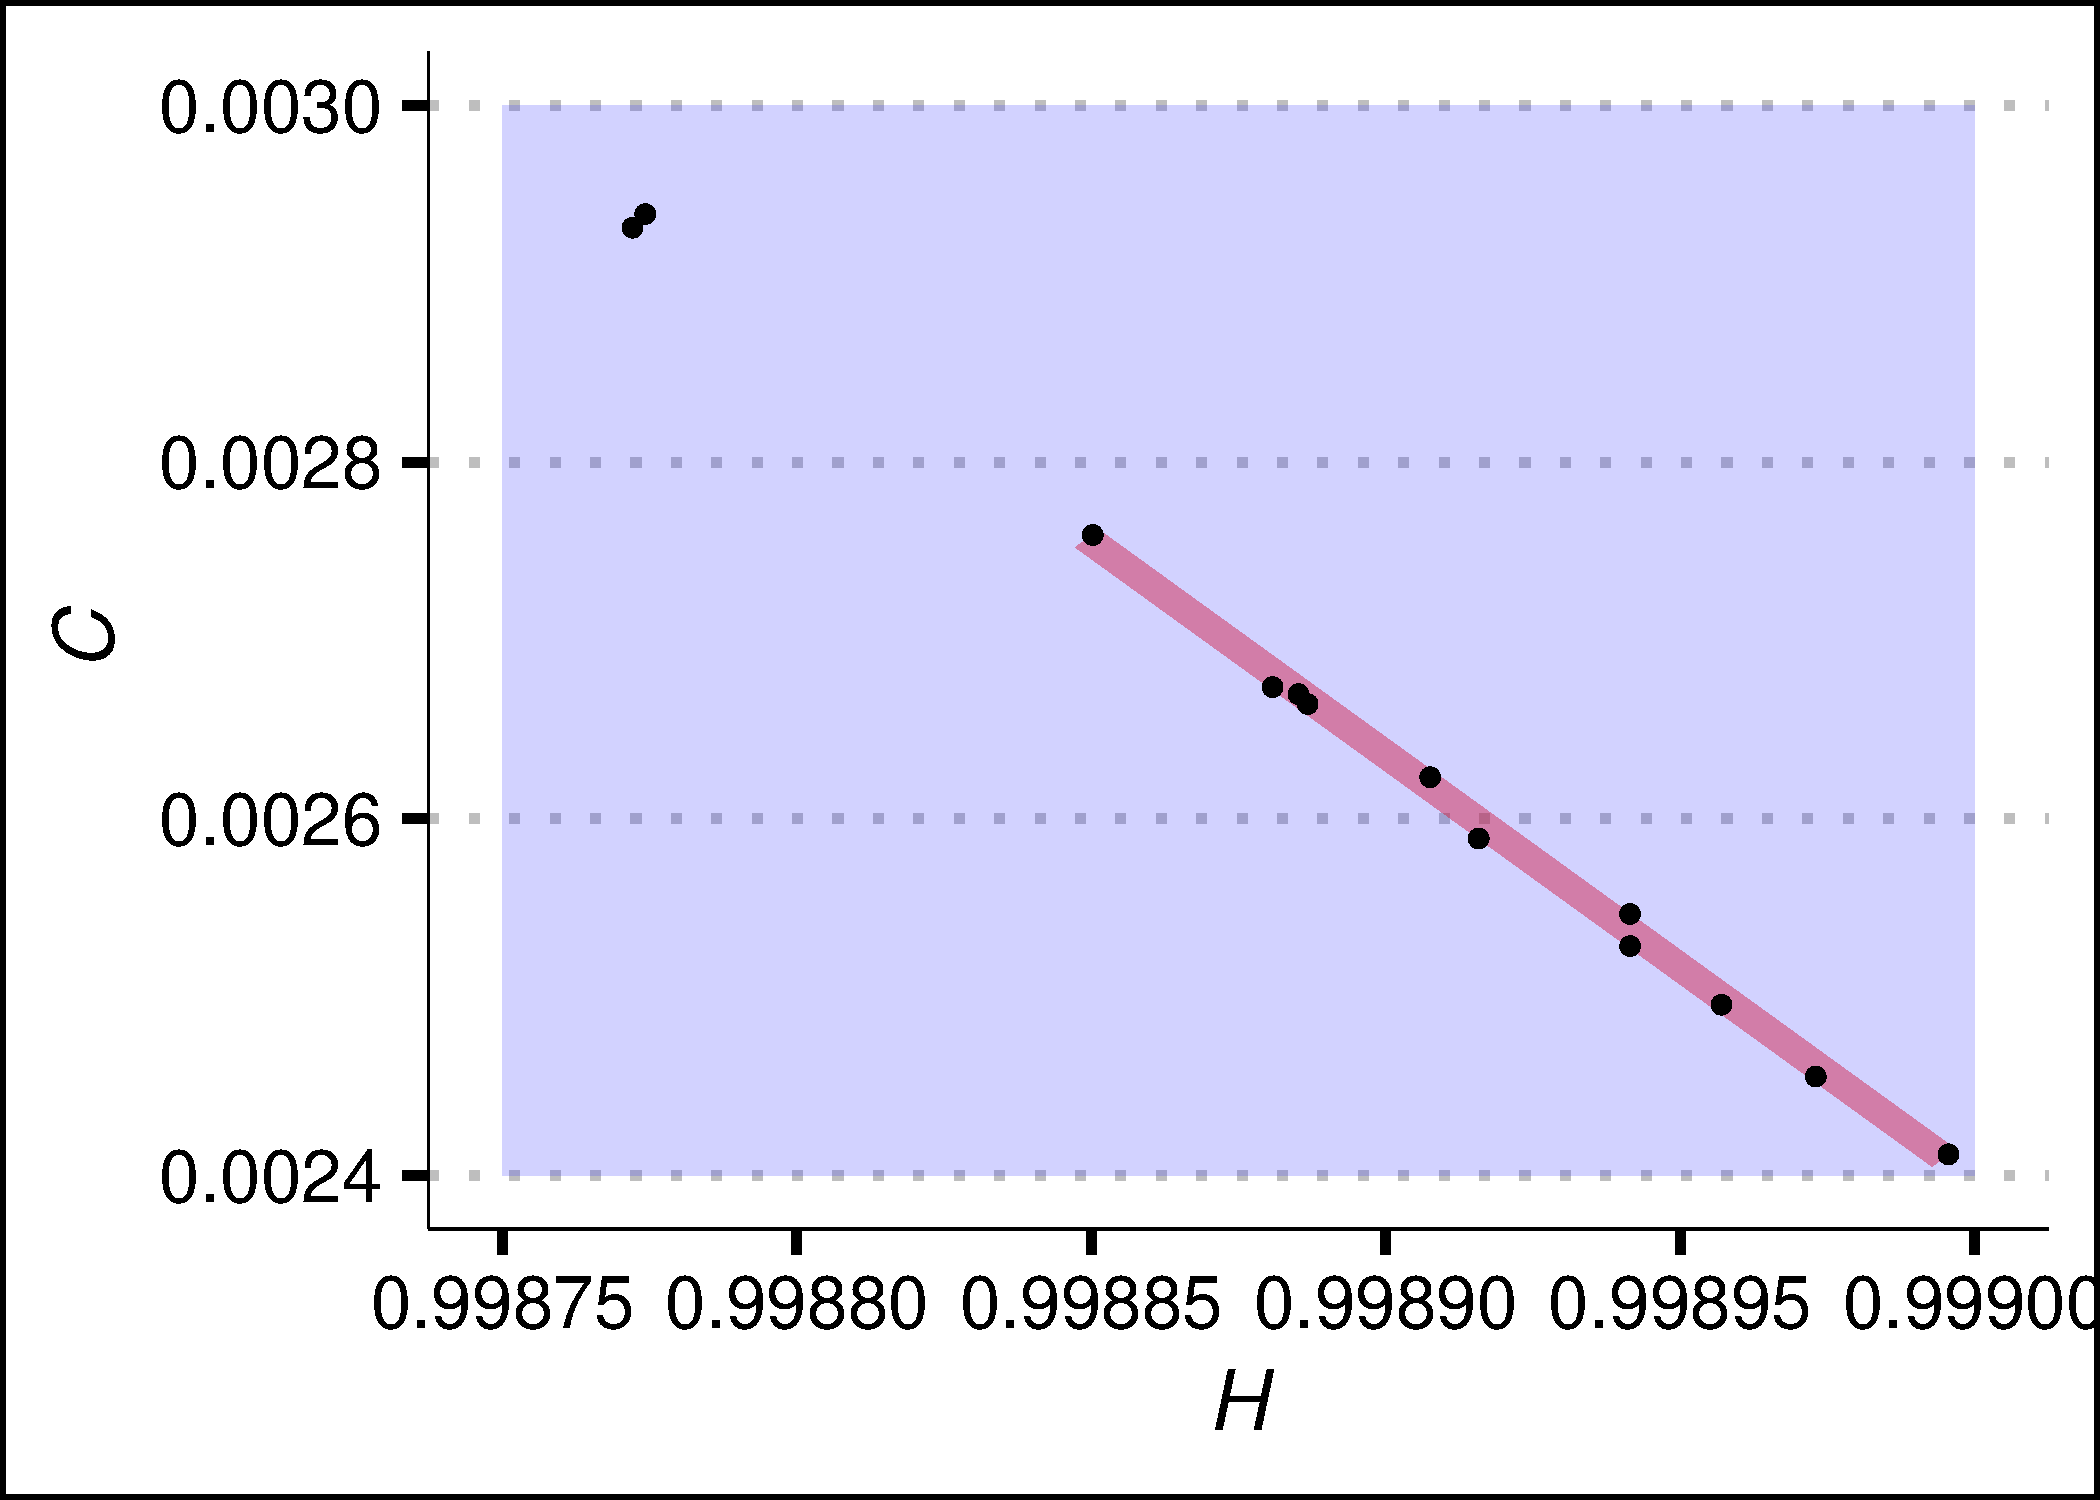
\includegraphics[width=.33\linewidth]{step3}}
	\caption{Outline of the methodology used for the construction of the confidence regions.}
	\label{fig:methodology}
\end{figure}

Algorithm~\ref{Algo:ConfidenceRegions} provides details on how we obtain the confidence regions, defined by a set of points $\bm P_1, \bm P_2, \bm P_2, \bm P_4$, for each $D\in \mathcal D$, each $T\in \mathcal T$, and each significance level $\alpha$.
We also obtain the ``emblematic point'' $\bm P'$, a kind of median point in the $H\times C$ plane for each situation.

\begin{algorithm}[hbt]
	\SetKwInOut{Input}{input}\SetKwInOut{Output}{output}
	\Input{A data base of true random values}
	\Input{The desired values of embedding dimension $\mathcal D$, sequence length $\mathcal T$, and confidence levels $\mathcal A$}
	\Output{Confidence regions as points in the $H\times C$ plane}
	\For{each $D\in \mathcal D$}{
		\For{each $T\in \mathcal T$}{
			\For{each $n=1,2,\dots,N$}{
				build the time series $p_n$ with unused values from the data base\;
				compute the point $(h_n,c_n)$ in the $H\times C$ plane that corresponds to $p_n$\; 
			}
			obtain $\text{PC}(D,T)$, the principal components transformation based on the points $(h_1,c_1),(h_2,c_2),\dots,(h_N,c_N)$, and its inverse $\text{PC}^{-1}(D,T)$\;
			%
			apply $\text{PC}(D,T)$ to the points $(h_1,c_1),(h_2,c_2),\dots,(h_N,c_N)$, and obtain $(u_1,v_1),(u_2,v_2),\dots,(u_N,v_N)$\;
			%
			find the indexes $\bm r=(r_1,r_2,\dots,r_N)$ that sort the values of the first principal component $\bm u=(u_1,u_2,\dots,u_N)$ in ascending order\;
			%
			find the point $(u,v)$ whose first principal component is the median: $(u_{r_{(N+1)/2}}, \cdot)$\;
			%
			apply the inverse principal components transformation $\text{PC}^{-1}(D,T)$ to $(u,v)$, and obtain $\bm P'=(h',v')$; call the corresponding time series ``emblematic time series''\;
			\Return{$\bm P'$}\;
			%
			\For{each confidence level $\alpha \in \mathcal A$}{
				find the point $(u,v)$ whose first principal component is the quantile $\alpha/2$: $(u_{r_{[N\alpha/2]}}, \cdot)$\;
				%
				find the point $(u,v)$ whose first principal component is the quantile $1-\alpha/2$: $(u_{r_{[N(1-\alpha/2)]}}, \cdot)$\;
				%
				the values $u_{r_{[N\alpha/2]}}$ and $u_{r_{[N(1-\alpha/2)]}}$ are the rightmost and leftmost bounds of the box, respectively\;
				%
				the bottom bound of the box is the smallest second principal component value whose first principal component is at least $u_{r_{[N\alpha/2]}}$; denote this value $v_{\min}$\;
				%
				the top bound of the box is the largest second principal value whose first principal component is at most $u_{r_{[N(1-\alpha/2)]}}$; denote this value $v_{\max}$\;
				%
				the corners of the box are 
				$(u_{r_{[N\alpha/2]}}, v_{\min})$, 
				$(u_{r_{[N\alpha/2]}}, v_{\max})$, 
				$(u_{r_{[N(1-\alpha/2)]}}, v_{\min})$ and 
				$(u_{r_{[N(1-\alpha/2)]}},v_{\max})$\;
				%
				apply the inverse principal components transformation $\text{PC}^{-1}(D,T)$ to these corners obtaining $\bm P_1=(h_{v_1}, c_{v_1})$, $\bm P_2=(h_{v_2},h_{v_2})$, $\bm P_3=(h_{v_3}, c_{v_3})$ and $\bm P_4=(h_{v_4},c_{v_4})$\;
				\Return{$\bm P_1$, $\bm P_2$, $\bm P_3$, $\bm P_4$}\;
			}
		}
	}
	\caption{Determination of confidence regions and emblematic time series}\label{Algo:ConfidenceRegions}
\end{algorithm}


%The visual representation of the proposed technique can be seen in Fig.~\ref{fig:methodology}.

These confidence regions obtained provide a powerful tool to make binary assessments about the adequacy of a given time series $\bm x$ to the null hypothesis $\mathcal H_0$ that it is white noise.
More generally, we are interested in obtaining the $p$-value of $\bm x$ under $\mathcal H_0$.
We present a procedure to obtain an approximate $p$-value based on the evidence collected to build the confidence regions.

The procedure operates on the principal components space and consists of measuring the closeness between the ``emblematic point'' and the observed point.
We are given a time series $\bm x$ of size $T$, and we want its $p$-value when contrasted with TWNRS of the same size at embedding dimension $D$.
We use $N$ TWNRS of size $T$, compute their points in the $H\times C$ plane, and project them to the corresponding principal components space.
We then do the same with $\bm x$, and obtain a new point $(u_x,v_x)$.
The closer $\bm x$ is to the emblematic time series, the larger its $p$-value.
Assume that the emblematic time series is represented by $(u,v)$ in the principal components space.
We measure this closeness by building a box around $(u_x,v_x)$ that contains $(u,v)$; assume that $u_x>u$, then:
\begin{enumerate}
	\item the right side of the box is the smallest $u_j$ which is larger that $u_x$; assume it corresponds to the quantile $\eta_u$ of $\utilde u = (u_1,u_2,\dots, u_N)$. By definition, $\eta_u\geq 1/2$.
	%
	\item the left side of the box is the $1-\eta_u$ quantile of $\utilde u$.
	%
	\item the top side of the box is the smallest $v_j$ which is larger that $v_x$; assume it corresponds to the quantile $\eta_v$ of $\utilde v = (v_1,v_2,\dots, v_N)$. By definition, $\eta_v\geq 1/2$.
	%
	\item the bottom side of the box is the $1-\eta_v$ quantile of $\utilde v$.
\end{enumerate}
Fig.~\ref{fig:methodologyPvalue} illustrates theses steps.

The definition of the box for the case $u_x<u$ follows naturally, and is described in Algorithm~\ref{Algo:p-value}.
With this approach, we obtain the smallest box that (i)~contains the new point, and (ii)~is defined by observed points from TRWNS.

Such boxes are less prone to distortions in this space since the distribution of the points becomes less asymmetric than in the $H\times C$ plane; cf.\ Fig.~\ref{fig:HC-PCA}.
Algorithm~\ref{Algo:p-value} shows the details.

\begin{figure}[hbt]
	\centering
	\subfloat[Points produced by TRWNSs in the space of principal components.\label{fig:v1}]{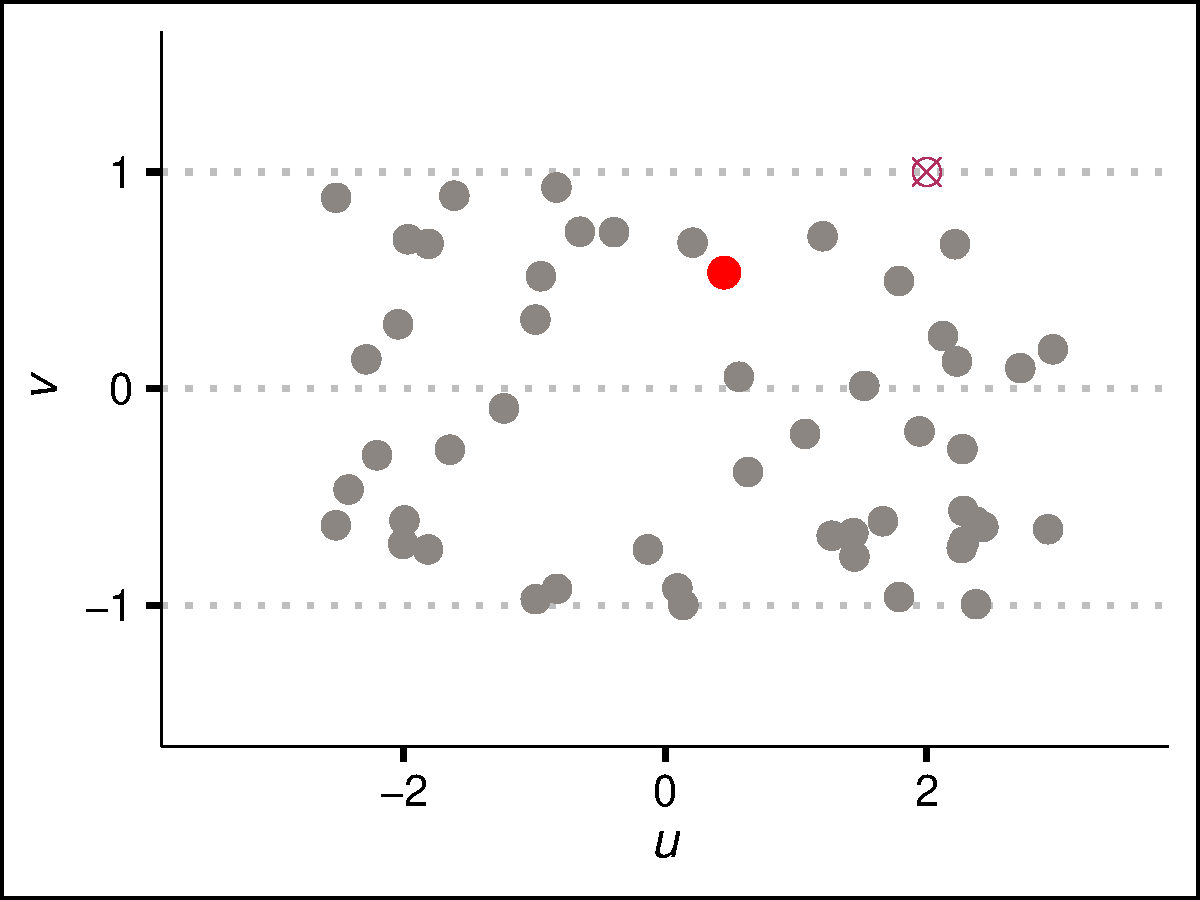
\includegraphics[width=.33\linewidth]{PvalueStep1}}
	\subfloat[Points whose first principal component is the median (red) and quantiles of order $\eta_u$ and $1-\eta_u$ (green).\label{fig:methodologyPvalue2}]{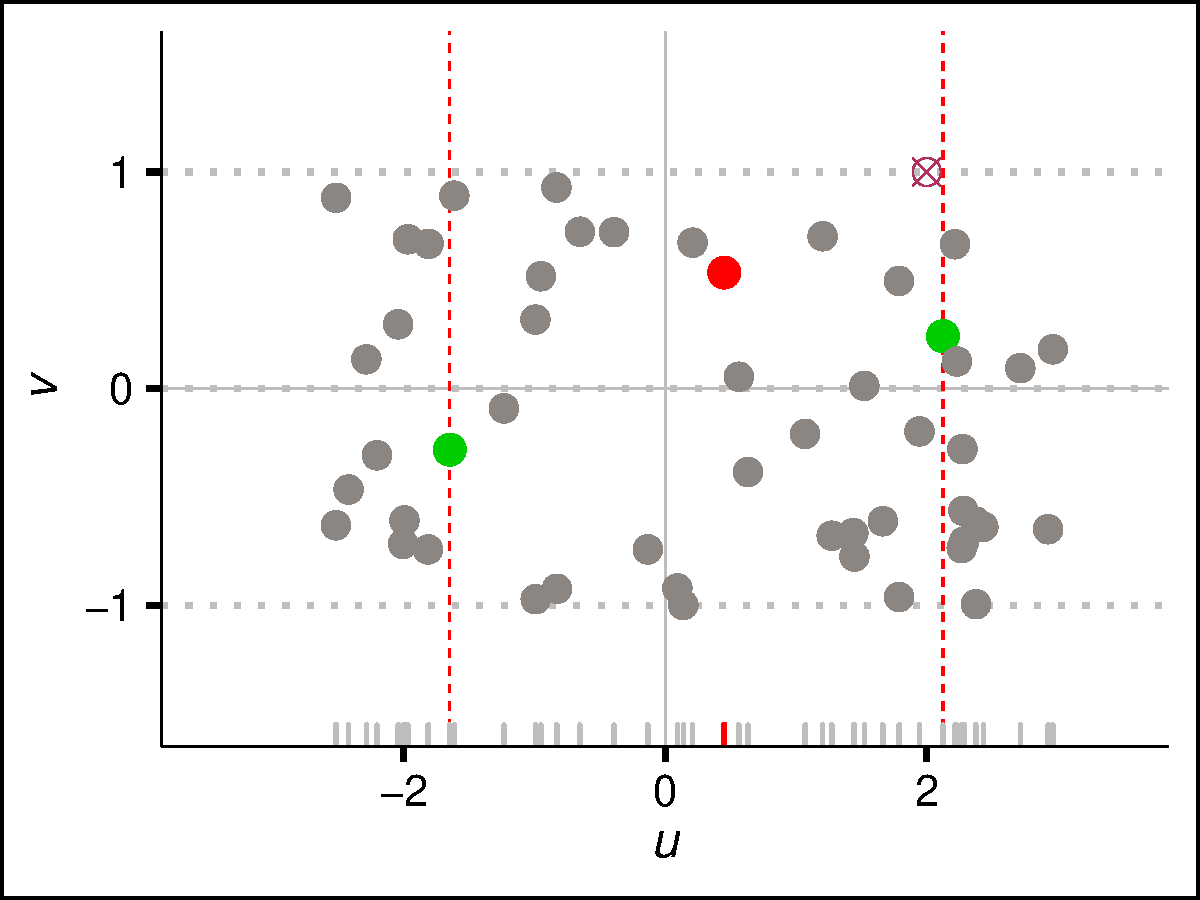
\includegraphics[width=.33\linewidth]{PvalueStep2}}
	\subfloat[The $p$-value of the new point is the proportion of points outside the box.\label{fig:methodologyPvalue3}]{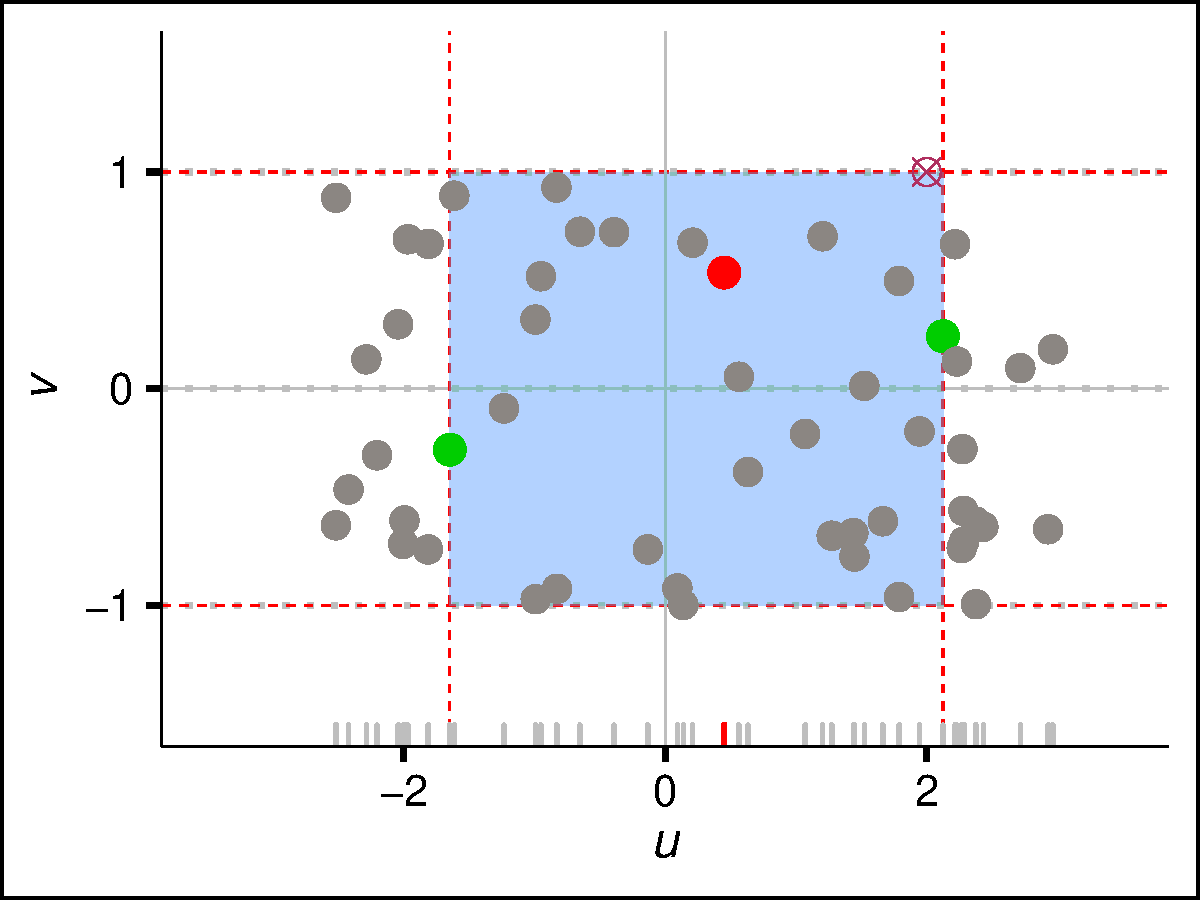
\includegraphics[width=.33\linewidth]{PvalueStep3}}
	\caption{Outline of the methodology used to calculate the $p$-value. The new point is denoted as a crossed circle.}
	\label{fig:methodologyPvalue}
\end{figure}

\begin{comment}
The empirical $p$-value of $\bm x'$ for the null hypothesis is given by the percentage of points outside the lowest confidence region obtained by the reference points to which $\bm x'$ belongs.
Therefore, it can be achieved by the following steps:
\begin{enumerate}
\item Compute $(h',c')$ the point in the $H\times C$ plane produced by $\bm x'$;
\item Compute $b_{T,D}(\bm x')$: the smallest box which contains $(h',c')$ using the $M$ reference points;
\item The empirical $p$-value of $\bm x'$ is obtained by the percentage of reference points outside $b_{T,D}(\bm x')$.
\end{enumerate}
Thus, we can verify that:
\begin{itemize}
\item the smallest $b_{T,D}(\bm x')$ is observed when $(h',c')$ ``coincides'' with the point produced by the emblematic sequence, in other words, point whose first principal component is the median of the $M$ reference points, and
\item the largest box is any box associated to $(h',c')$ ``outside'' the largest box produced by the $M$ reference points.
\end{itemize}
Assuming the critical value $\alpha = 0.05$, we obtain:
\begin{equation*}
p-\text{value} \geq \alpha, \text{ the null hypothesis should not be rejected}.
\end{equation*}
\end{comment}

\begin{algorithm}[hbt]
	\SetKwInOut{Input}{input}\SetKwInOut{Output}{output}
	\Input{The sequence $\bm x$ of length $T$ to be contrasted to the null hypothesis $\mathcal H_0$ that it is adherent to white noise}
	\Input{The embedding dimension $D$}
	\Input{$N$ points $(h_1,c_1),(h_2,c_2),\dots,(h_N,c_N)$ of true white noise series of length $T$;
		the principal components tranformation $\text{PC}(D,T)$ induced by these points;	
		the points projected onto the $H\times C$ plane: $(u_1,v_1),(u_2,v_2),\dots,(u_N,v_N)$}
	\Output{An approximate $p$-value}
	find the point $(u,v)$ whose first principal component is the median: $(u_{r_{(N+1)/2}}, \cdot)$\;
	find the point $(h,c)$ of the sequence $\bm x$\;
	find the projection $(u_x,v_x)$ of $(h,c)$ onto the principal components space using $\text{PC}(D,T)$\;	
	\eIf{$u_x > u$}
	{ $u_{r_{[N(1-\alpha/2)]}}$ is defined as the smallest element larger than $u_x$\;
		$u_{r_{[N\alpha/2]}} \leftarrow 2u - u_{r_{[N(1-\alpha/2)]}}$\;
	}
	{
		\eIf{$u_x < u$}
		{ $u_{r_{[N\alpha/2]}}$ is the largest minor element of $u_x$\;
			$u_{r_{[N(1-\alpha/2)]}} \leftarrow 2u - u_{r_{[N\alpha/2]}}$\;
		}
		{ $u_{r_{[N\alpha/2]}}$ and $u_{r_{[N(1-\alpha/2)]}}$ is equal to $u$, the median point of the first principal component\; 
		}
	}
	obtain the maximum values of the second component whose values of the first principal component are at least $u_{r_{[N\alpha/2]}}$ and at most $u_{r_{[N(1-\alpha/2)]}}$ and denote it $v_{\max}$\;
	obtain the minimum values of the second component whose values of the first principal component are at least $u_{r_{[N\alpha/2]}}$ and at most $u_{r_{[N(1-\alpha/2)]}}$ and denote it $v_{\min}$\;
	the corners of the box $b_{\alpha}(h,c)$ are 
	$(u_{r_{[N\alpha/2]}}, v_{\min})$, 
	$(u_{r_{[N\alpha/2]}}, v_{\max})$, 
	$(u_{r_{[N(1-\alpha/2)]}}, v_{\min})$ and 
	$(u_{r_{[N(1-\alpha/2)]}}, v_{\max})$\;
	%find $b_{T,D}(h,c)$: the smallest box centered at $(h',c')$ which contains $\text{PC}(D,T)(h,c)$\;
	count $n_{\bm x}$, the number of points out of the $N$ points which belong to $b_{\alpha}(h,c)$\;
	\Return{$1-n_{\bm x}/N$}
	\caption{Determination of the $p$-value of the sequence $\bm x$ under $\mathcal H_0$}\label{Algo:p-value}
\end{algorithm}

\section{Results}\label{Sec:Results}

\subsection{Empirical confidence regions}

Tables~\ref{Tab:Points1k} and~\ref{Tab:Points50k} list the coordinates in the $H\times C$ plane
of the emblematic point $\bm P'$ and of the four points $\bm P_1,\bm P_2,\bm P_3,\bm P_4$ that define the confidence regions at \SI{90}{\percent}, \SI{95}{\percent}, \SI{99}{\percent}, and \SI{99.9}{\percent}, 
for $D=3,4,5,6$ and $N=1000,50000$, .
The points are presented counterclockwise, starting with the one with the largest complexity. 

\begin{comment}
\begin{table}[hbt]
\caption{Coordinates in the $H\times C$ plane of the emblematic series and the points that define the confidence regions at \SI{90}{\percent}, \SI{95}{\percent}, \SI{99}{\percent}, and \SI{99.9}{\percent} for $D=3,4,5,6$ and $N=1000,50000$}\label{Tab:Points}
\centering
\begin{tabular}{rcllllllll}
\toprule
& & \multicolumn{8}{c}{$N$}\\ \cmidrule(lr){3-10}
& & \multicolumn{4}{c}{$1000$} & \multicolumn{4}{c}{$50000$}\\ \cmidrule(lr){3-6} \cmidrule(lr){7-10}
$D$ & Point & \SI{90}{\percent} & \SI{95}{\percent} & \SI{99}{\percent} & \SI{99.9}{\percent} & \SI{90}{\percent} & \SI{95}{\percent} & \SI{99}{\percent} & \SI{99.9}{\percent}\\ \cmidrule(lr){3-3} \cmidrule(lr){4-4} \cmidrule(lr){5-5} \cmidrule(lr){6-6} \cmidrule(lr){7-7} \cmidrule(lr){8-8} \cmidrule(lr){9-9} \cmidrule(lr){10-10}
$3$ & $\bm P'$ & \multicolumn{4}{c}{$h',c'$} & \multicolumn{4}{c}{$h',c'$}\\
& $\bm P_1$ & $(0.9973334, 0.0025601)$ & $(0.9967311, 0.0031343)$ & $(0.9953009, 0.0045054)$ & $(0.9931825, 0.0065387)$ & $(0.9999489, \num[scientific-notation=true]{5.06e-05})$ & $(0.9999384, \num[scientific-notation=true]{6.11e-05})$ & $(0.9999079, \num[scientific-notation=true]{9.11e-05})$ & $(0.9998625, 0.0001361)$\\
& $\bm P_2$ & $(0.9974047, 0.0026304)$ & $(0.9968219, 0.0032238)$ & $(0.9954349, 0.0046375)$ & $(0.9933704, 0.006724)$ & $(0.9999487, \num[scientific-notation=true]{5.04e-05})$ & $(0.9999382, \num[scientific-notation=true]{6.09e-05})$ & $(0.9999077, \num[scientific-notation=true]{9.09e-05})$ & $(0.9998622, 0.0001358)$\\
& $\bm P_3$ & $(0.9999497, 0)$ & $(0.9999398, 0)$ & $(0.9999203, 0)$ & $(0.9998925, 0)$ & $(0.9999998, \num[scientific-notation=true]{4e-07})$ & $(0.9999994, \num[scientific-notation=true]{9e-07})$ & $(0.9999982, \num[scientific-notation=true]{2e-06})$ & $(0.9999973, \num[scientific-notation=true]{3e-06})$\\
& $\bm P_4$ & $(1, \num[scientific-notation=true]{5.17e-05})$ & $(1, \num[scientific-notation=true]{6.12e-05})$ & $(1, \num[scientific-notation=true]{8.45e-05})$ & $(1, 0.0001104)$ & $(0.9999996, \num[scientific-notation=true]{2e-07})$ & $(0.9999991, \num[scientific-notation=true]{7e-07})$ & $(0.999998, \num[scientific-notation=true]{1.8e-06})$ & $(0.999997, \num[scientific-notation=true]{2.7e-06})$\\ \midrule
$4$ & $\bm P'$ & \multicolumn{4}{c}{$h',c'$} & \multicolumn{4}{c}{$h',c'$}\\
& $\bm P_1$ & $(0.994364, 0.0081246)$ & $(0.9937138, 0.0089796)$ & $(0.9922575, 0.0108947)$ & $(0.9902578, 0.0135243)$ & $(0.9999684, \num[scientific-notation=true]{3.98e-05})$ & $(0.9999725, \num[scientific-notation=true]{3.44e-05})$ & $(0.9999783, \num[scientific-notation=true]{2.68e-05})$ & $(0.9999833, \num[scientific-notation=true]{2.02e-05})$ \\
& $\bm P_2$ & $(0.9939234, 0.0075452)$ & $(0.9932534, 0.0083741)$ & $(0.9917308, 0.0102022)$ & $(0.9897312, 0.0128318)$ & $(0.9999696, \num[scientific-notation=true]{4.13e-05})$ & $(0.9999737, \num[scientific-notation=true]{3.6e-05})$ & $(0.9999795, \num[scientific-notation=true]{2.83e-05})$ & $(0.9999845, \num[scientific-notation=true]{2.18e-05})$ \\
& $\bm P_3$ & $(0.9994791, 0.0013982)$ & $(0.9991609, 0.0018166)$ & $(0.9987924, 0.0023012)$ & $(0.9985727, 0.0025901)$ & $(0.9998075, 0.0002508)$ & $(0.9998506, 0.0001942)$ & $(0.9998756, 0.0001615)$ & $(0.9998889, 0.000144)$ \\
& $\bm P_4$ & $(0.9990385, 0.0008188)$ & $(0.9987005, 0.0012111)$ & $(0.9982658, 0.0016087)$ & $(0.9980461, 0.0018976)$ & $(0.9998087, 0.0002524)$ & $(0.9998518, 0.0001958)$ & $(0.9998768, 0.000163)$ & $(0.9998901, 0.0001456)$ \\ \midrule
$5$ & $\bm P'$ & \multicolumn{4}{c}{$h',c'$} & \multicolumn{4}{c}{$h',c'$}\\
& $\bm P_1$ & $(0.9811818, 0.0321294)$ & $(0.9801289, 0.0340045)$ & $(0.977917, 0.0377295)$ & $(0.9753326, 0.0425299)$ & $(0.9998172, 0.0003232)$ & $(0.9998259, 0.0003075)$ & $(0.9998428, 0.0002774)$ & $(0.9998573, 0.0002517)$ \\
& $\bm P_2$ & $(0.9827429, 0.0350291)$ & $(0.9817117, 0.0369446)$ & $(0.9796031, 0.0408613)$ & $(0.9770187, 0.0456617)$ & $(0.9998194, 0.0003273)$ & $(0.9998282, 0.0003116)$ & $(0.999845, 0.0002814)$ & $(0.9998593, 0.0002553)$ \\
& $\bm P_3$ & $(0.9919707, 0.0120896)$ & $(0.9909376, 0.0139279)$ & $(0.9898161, 0.0156277)$ & $(0.9892599, 0.0166608)$ & $(0.9994812, 0.0009246)$ & $(0.9996371, 0.0006455)$ & $(0.9996703, 0.0005862)$ & $(0.9996884, 0.000554)$ \\
& $\bm P_4$ & $(0.9935319, 0.0149893)$ & $(0.9925204, 0.016868)$ & $(0.9915021, 0.0187595)$ & $(0.9909459, 0.0197926)$ & $(0.9994834, 0.0009286)$ & $(0.9996394, 0.0006495)$ & $(0.9996725, 0.0005901)$ & $(0.9996904, 0.0005576)$ \\ \midrule
$6$ & $\bm P'$ & \multicolumn{4}{c}{$h',c'$} & \multicolumn{4}{c}{$h',c'$}\\
& $\bm P_1$ & $(0.9121895, 0.2201993)$ & $(0.9105951, 0.2239294)$ & $(0.9105951, 0.2239294)$ & $(0.9077672, 0.2305874)$ & $(0.9990169, 0.002336)$ & $(0.9990368, 0.002288)$ & $(0.9990736, 0.0021997)$ & $(0.9991069, 0.0021197)$ \\
& $\bm P_2$ & $(0.9146048, 0.2260776)$ & $(0.9130413, 0.2298829)$ & $(0.9130413, 0.2298829)$ & $(0.9102595, 0.2366531)$ & $(0.9990249, 0.0023554)$ & $(0.9990449, 0.0023074)$ & $(0.9990817, 0.0022191)$ & $(0.999115, 0.0021392)$ \\
& $\bm P_3$ & $(0.9443868, 0.1418373)$ & $(0.9419202, 0.1476904)$ & $(0.9396577, 0.1531967)$ & $(0.9383611, 0.1561279)$ & $(0.9978983, 0.0050219)$ & $(0.998714, 0.0030633)$ & $(0.998765, 0.0029407)$ & $(0.9987884, 0.0028845)$ \\
& $\bm P_4$ & $(0.9468021, 0.1477156)$ & $(0.9443663, 0.1536439)$ & $(0.9421039, 0.1591502)$ & $(0.9408534, 0.1621937)$ & $(0.9979064, 0.0050413)$ & $(0.998722, 0.0030827)$ & $(0.9987731, 0.0029601)$ & $(0.9987965, 0.0029039)$ \\ \bottomrule
\end{tabular}
\end{table}
\end{comment}

\begin{table}[hbt]
	\caption{Coordinates in the $H\times C$ plane of the emblematic series and the points that define the confidence regions at \SI{90}{\percent}, \SI{95}{\percent}, \SI{99}{\percent}, and \SI{99.9}{\percent} for $D=3,4,5,6$ and $N=1000$}\label{Tab:Points1k}
	\centering
	\begin{tabular}{rccccc}
		\toprule
		%& & \multicolumn{4}{c}{$N$}\\ 
		%\cmidrule(lr){3-6}
		& & \multicolumn{4}{c}{$N = 1000$}\\ 
		\cmidrule(lr){3-6} 
		$D$ & Point & \SI{90}{\percent} & \SI{95}{\percent} & \SI{99}{\percent} & \SI{99.9}{\percent}\\ 
		\cmidrule(lr){3-3} 
		\cmidrule(lr){4-4} 
		\cmidrule(lr){5-5} 
		\cmidrule(lr){6-6} 
		$3$ & $\bm P'$ & \multicolumn{4}{c}{$(0.9992089,0.0007800)$}\\
		& $\bm P_1$ & $(0.9973334, 0.0025601)$ & $(0.9967311, 0.0031343)$ & $(0.9953009, 0.0045054)$ & $(0.9931825, 0.0065387)$\\
		& $\bm P_2$ & $(0.9974047, 0.0026304)$ & $(0.9968219, 0.0032238)$ & $(0.9954349, 0.0046375)$ & $(0.9933704, 0.006724)$\\
		& $\bm P_3$ & $(0.9999497, 0)$ & $(0.9999398, 0)$ & $(0.9999203, 0)$ & $(0.9998925, 0)$\\
		& $\bm P_4$ & $(1, \num[scientific-notation=true]{5.17e-05})$ & $(1, \num[scientific-notation=true]{6.12e-05})$ & $(1, \num[scientific-notation=true]{8.45e-05})$ & $(1, 0.0001104)$\\ 
		\midrule
		$4$ & $\bm P'$ & \multicolumn{4}{c}{$(0.9967032, 0.0043297)$} \\
		& $\bm P_1$ & $(0.994364, 0.0081246)$ & $(0.9937138, 0.0089796)$ & $(0.,9922575 0.0108947)$ & $(0.9902578, 0.0135243)$\\
		& $\bm P_2$ & $(0.9939234, 0.0075452)$ & $(0.9932534, 0.0083741)$ & $(0.9917308, 0.0102022)$ & $(0.9897312, 0.0128318)$\\
		& $\bm P_3$ & $(0.9994791, 0.0013982)$ & $(0.9991609, 0.0018166)$ & $(0.9987924, 0.0023012)$ & $(0.9985727, 0.0025901)$\\
		& $\bm P_4$ & $(0.9990385, 0.0008188)$ & $(0.9987005, 0.0012111)$ & $(0.9982658, 0.0016087)$ & $(0.9980461, 0.0018976)$\\ 
		\midrule
		$5$ & $\bm P'$ & \multicolumn{4}{c}{$(0.9864873, 0.0245632)$}\\
		& $\bm P_1$ & $(0.9811818, 0.0321294)$ & $(0.9801289, 0.0340045)$ & $(0.977917, 0.0377295)$ & $(0.9753326, 0.0425299)$\\
		& $\bm P_2$ & $(0.9827429, 0.0350291)$ & $(0.9817117, 0.0369446)$ & $(0.9796031, 0.0408613)$ & $(0.9770187, 0.0456617)$\\
		& $\bm P_3$ & $(0.9919707, 0.0120896)$ & $(0.9909376, 0.0139279)$ & $(0.9898161, 0.0156277)$ & $(0.9892599, 0.0166608)$\\
		& $\bm P_4$ & $(0.9935319, 0.0149893)$ & $(0.9925204, 0.016868)$ & $(0.9915021, 0.0187595)$ & $(0.9909459, 0.0197926)$\\ 
		\midrule
		$6$ & $\bm P'$ & \multicolumn{4}{c}{$(0,9296429, 0.1841438)$}\\
		& $\bm P_1$ & $(0.9121895, 0.2201993)$ & $(0.9105951, 0.2239294)$ & $(0.9105951, 0.2239294)$ & $(0.9077672, 0.2305874)$\\
		& $\bm P_2$ & $(0.9146048, 0.2260776)$ & $(0.9130413, 0.2298829)$ & $(0.9130413, 0.2298829)$ & $(0.9102595, 0.2366531)$\\
		& $\bm P_3$ & $(0.9443868, 0.1418373)$ & $(0.9419202, 0.1476904)$ & $(0.9396577, 0.1531967)$ & $(0.9383611, 0.1561279)$\\
		& $\bm P_4$ & $(0.9468021, 0.1477156)$ & $(0.9443663, 0.1536439)$ & $(0.9421039, 0.1591502)$ & $(0.9408534, 0.1621937)$\\ 
		\bottomrule
	\end{tabular}
\end{table}


\begin{table}[hbt]
	\caption{Coordinates in the $H\times C$ plane of the emblematic series and the points that define the confidence regions at \SI{90}{\percent}, \SI{95}{\percent}, \SI{99}{\percent}, and \SI{99.9}{\percent} for $D=3,4,5,6$ and $N=50000$}\label{Tab:Points50k}
	\centering
	\begin{tabular}{rccccc}
		\toprule
		%& & \multicolumn{4}{c}{$N$}\\ 
		%\cmidrule(lr){3-6}
		& & \multicolumn{4}{c}{$N = 50000$}\\ 
		\cmidrule(lr){3-6} 
		$D$ & Point & \SI{90}{\percent} & \SI{95}{\percent} & \SI{99}{\percent} & \SI{99.9}{\percent}\\ 
		\cmidrule(lr){3-3} 
		\cmidrule(lr){4-4} 
		\cmidrule(lr){5-5} 
		\cmidrule(lr){6-6} 
		$3$ & $\bm P'$ & \multicolumn{4}{c}{$(0.9999853, \num[scientific-notation=true]{1.45e-05})$}\\
		& $\bm P_1$ & $(0.9999489, \num[scientific-notation=true]{5.06e-05})$ & $(0.9999384, \num[scientific-notation=true]{6.11e-05})$ & $(0.9999079, \num[scientific-notation=true]{9.11e-05})$ & $(0.9998625, 0.0001361)$\\
		& $\bm P_2$ & $(0.9999487, \num[scientific-notation=true]{5.04e-05})$ & $(0.9999382, \num[scientific-notation=true]{6.09e-05})$ & $(0.9999077, \num[scientific-notation=true]{9.09e-05})$ & $(0.9998622, 0.0001358)$\\
		& $\bm P_3$ & $(0.9999998, \num[scientific-notation=true]{4e-07})$ & $(0.9999994, \num[scientific-notation=true]{9e-07})$ & $(0.9999982, \num[scientific-notation=true]{2e-06})$ & $(0.9999973, \num[scientific-notation=true]{3e-06})$\\
		& $\bm P_4$ & $(0.9999996, \num[scientific-notation=true]{2e-07})$ & $(0.9999991, \num[scientific-notation=true]{7e-07})$ & $(0.999998, \num[scientific-notation=true]{1.8e-06})$ & $(0.999997, \num[scientific-notation=true]{2.7e-06})$\\ \midrule
		$4$ & $\bm P'$ & \multicolumn{4}{c}{$(0.9999394, \num[scientific-notation=true]{7.94e-05})$}\\
		& $\bm P_1$ & $(0.9999684, \num[scientific-notation=true]{3.98e-05})$ & $(0.9999725, \num[scientific-notation=true]{3.44e-05})$ & $(0.9999783, \num[scientific-notation=true]{2.68e-05})$ & $(0.9999833, \num[scientific-notation=true]{2.02e-05})$ \\
		& $\bm P_2$ & $(0.9999696, \num[scientific-notation=true]{4.13e-05})$ & $(0.9999737, \num[scientific-notation=true]{3.6e-05})$ & $(0.9999795, \num[scientific-notation=true]{2.83e-05})$ & $(0.9999845, \num[scientific-notation=true]{2.18e-05})$ \\
		& $\bm P_3$ & $(0.9998075, 0.0002508)$ & $(0.9998506, 0.0001942)$ & $(0.9998756, 0.0001615)$ & $(0.9998889, 0.000144)$ \\
		& $\bm P_4$ & $(0.9998087, 0.0002524)$ & $(0.9998518, 0.0001958)$ & $(0.9998768, 0.000163)$ & $(0.9998901, 0.0001456)$ \\ \midrule
		$5$ & $\bm P'$ & \multicolumn{4}{c}{$(0.9997616, 0.0004264)$}\\
		& $\bm P_1$ & $(0.9998172, 0.0003232)$ & $(0.9998259, 0.0003075)$ & $(0.9998428, 0.0002774)$ & $(0.9998573, 0.0002517)$ \\
		& $\bm P_2$ & $(0.9998194, 0.0003273)$ & $(0.9998282, 0.0003116)$ & $(0.999845, 0.0002814)$ & $(0.9998593, 0.0002553)$ \\
		& $\bm P_3$ & $(0.9994812, 0.0009246)$ & $(0.9996371, 0.0006455)$ & $(0.9996703, 0.0005862)$ & $(0.9996884, 0.000554)$ \\
		& $\bm P_4$ & $(0.9994834, 0.0009286)$ & $(0.9996394, 0.0006495)$ & $(0.9996725, 0.0005901)$ & $(0.9996904, 0.0005576)$ \\ \midrule
		$6$ & $\bm P'$ & \multicolumn{4}{c}{$(0.9989108, 0.0026093)$}\\
		& $\bm P_1$ & $(0.9990169, 0.002336)$ & $(0.9990368, 0.002288)$ & $(0.9990736, 0.0021997)$ & $(0.9991069, 0.0021197)$ \\
		& $\bm P_2$ & $(0.9990249, 0.0023554)$ & $(0.9990449, 0.0023074)$ & $(0.9990817, 0.0022191)$ & $(0.999115, 0.0021392)$ \\
		& $\bm P_3$ & $(0.9978983, 0.0050219)$ & $(0.998714, 0.0030633)$ & $(0.998765, 0.0029407)$ & $(0.9987884, 0.0028845)$ \\
		& $\bm P_4$ & $(0.9979064, 0.0050413)$ & $(0.998722, 0.0030827)$ & $(0.9987731, 0.0029601)$ & $(0.9987965, 0.0029039)$ \\ \bottomrule
	\end{tabular}
\end{table}

Fig.~\ref{fig:HC-PCA} shows the results for $T = 50000$ and $D = 3,6$ in the new principal components space, along with the quantiles of order $\SI{90}{\percent}$, $\SI{95}{\percent}$, $\SI{99}{\percent}$, and $\SI{99.9}{\percent}$.
We also show the projection of the $H \times C$ plane boundaries in this space, as well the median of each data set, the latter being represented as red dots.

\begin{figure}[hbt]
	\centering
	\subfloat[Points in the Principal Components plane for for $D=3$]{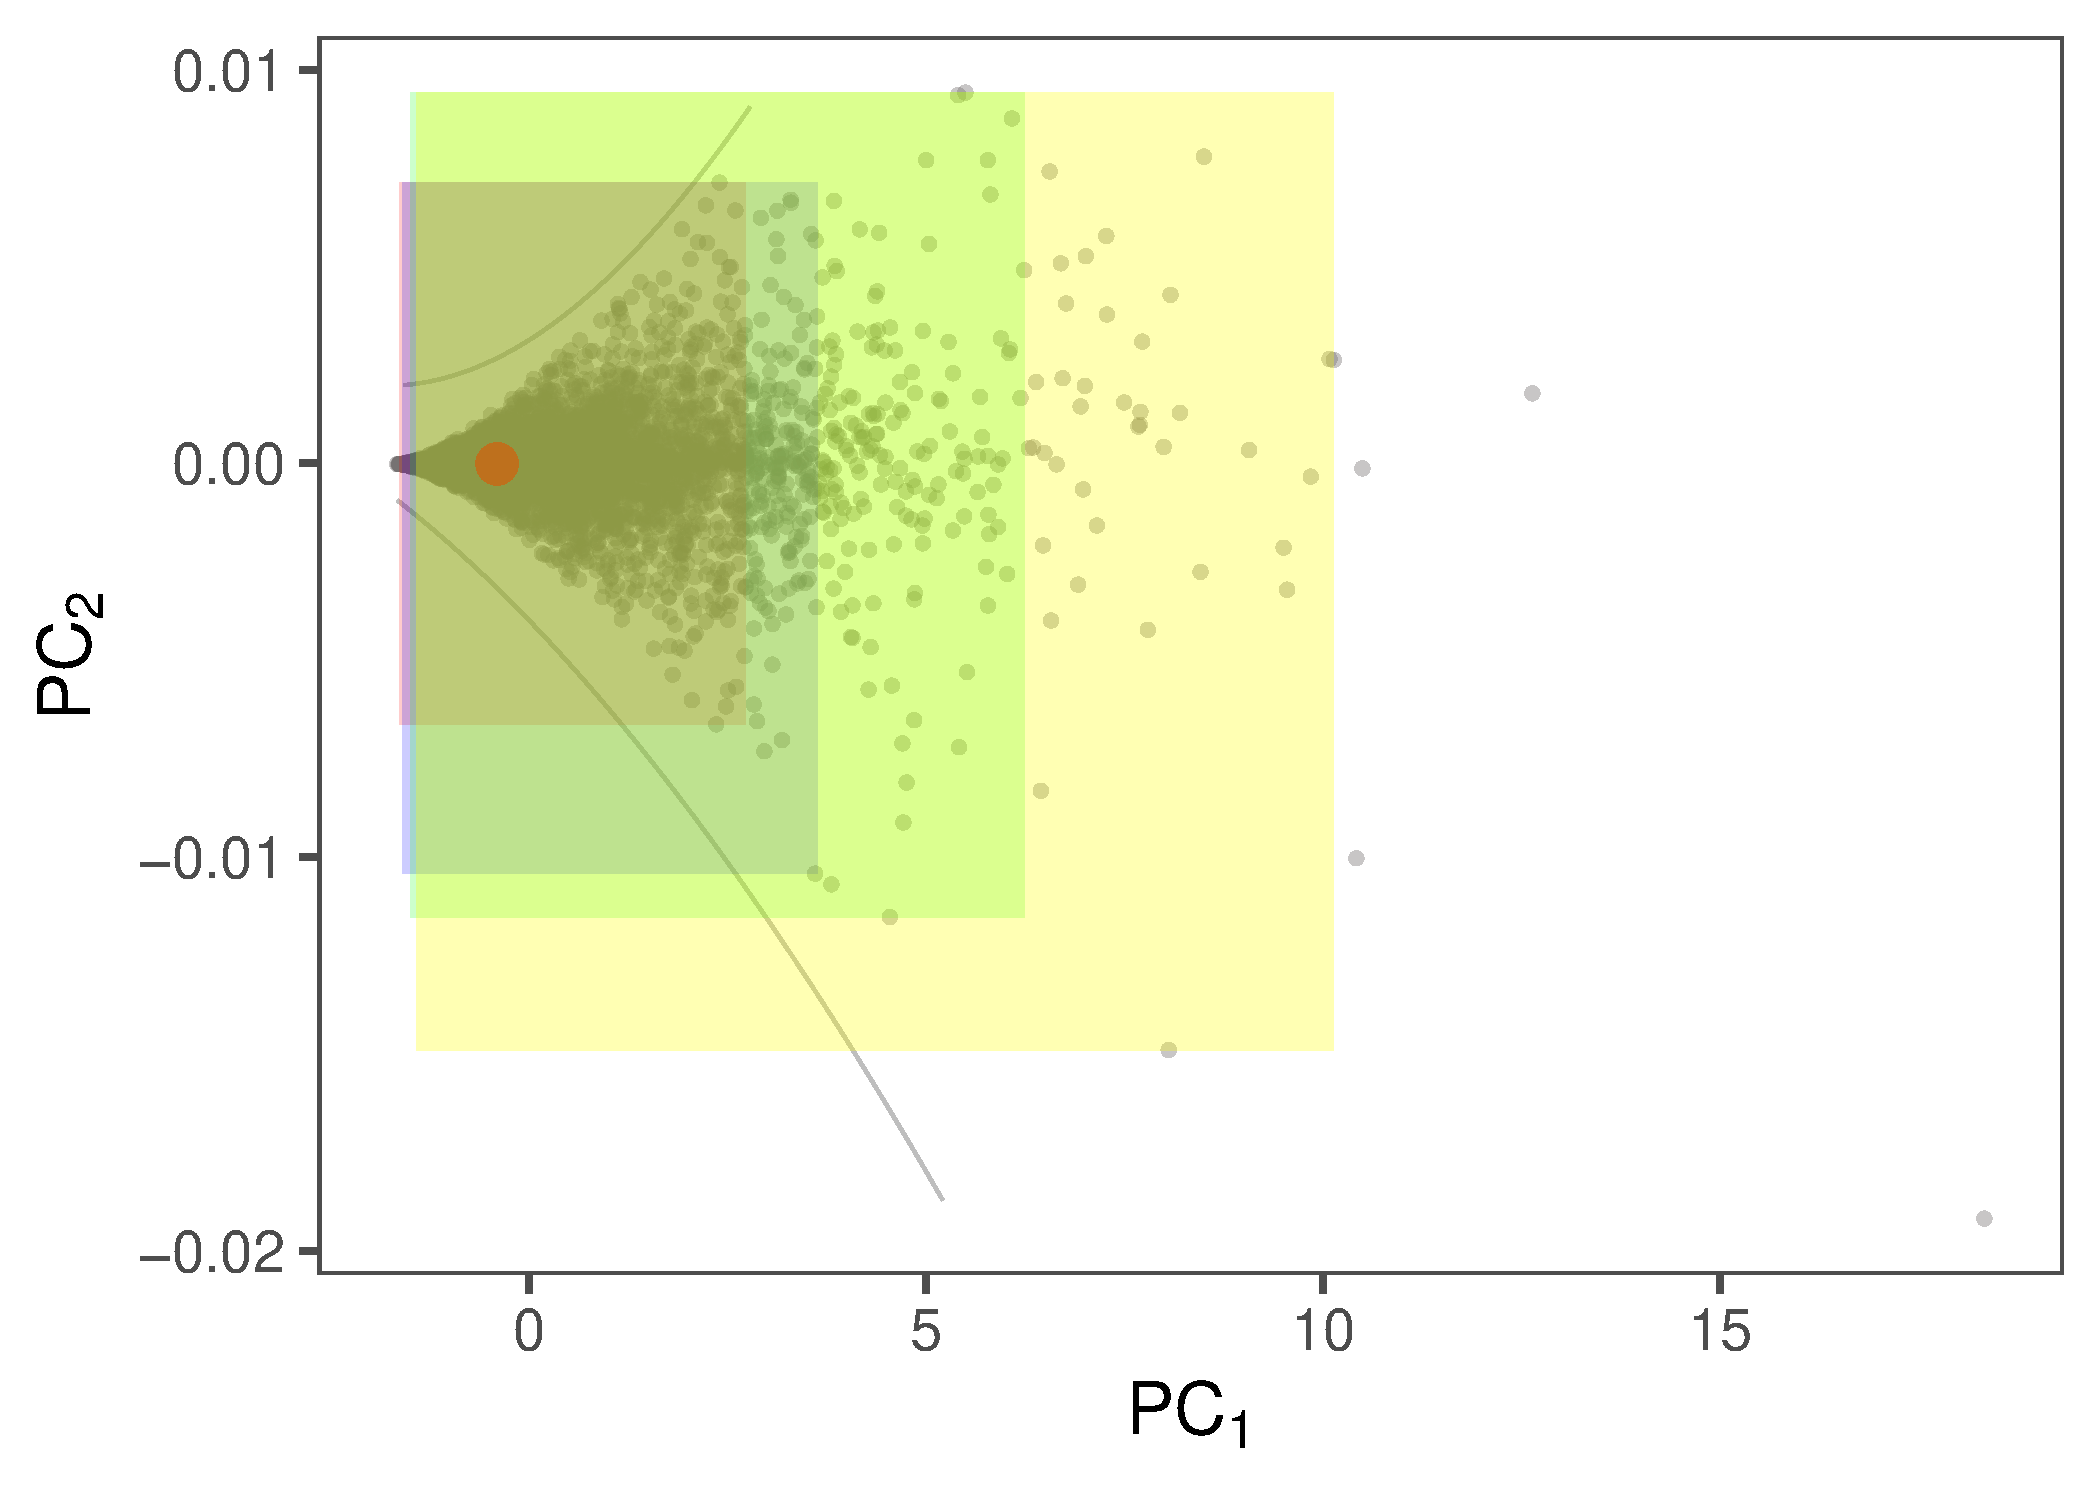
\includegraphics[width=.49\linewidth]{Figures/HC-PCA-Trozos-D3N50k}}
	\subfloat[Points in the Principal Components plane for for $D=6$]{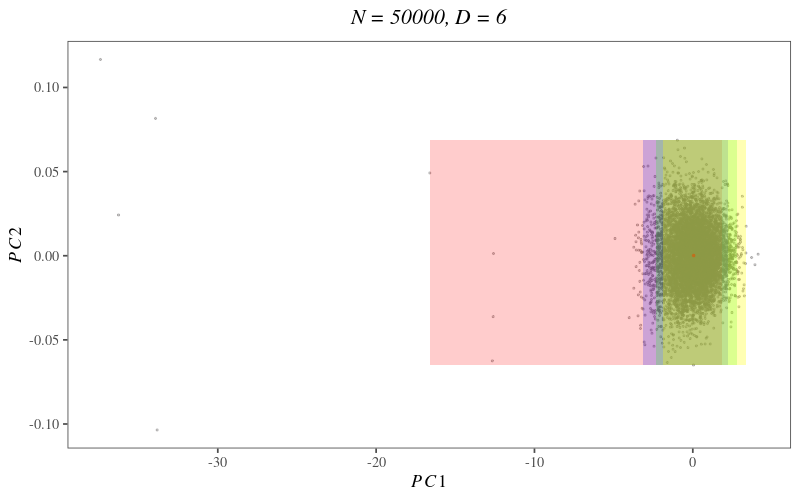
\includegraphics[width=.49\linewidth]{Figures/HC-PCA-Trozos-D6N50k}}
	\caption{Representation of true random white noise sequences of length $T = 50000$ in the PCA space for $D = 3$ and $D = 6$, and the quantiles of $\SI{90}{\percent}$, $\SI{95}{\percent}$, $\SI{99}{\percent}$, and $\SI{99.9}{\percent}$.}
	\label{fig:HC-PCA}
\end{figure} 

The confidence regions exceed the $H \times C$ boundaries, but this issue does not compromise the test's size since no points can be observed outside such boundaries.

Fig.~\ref{fig:HC-PCA} also shows that the data are not evenly distributed among the axes of the first principal component.
They tend to concentrate close to the point that corresponds to $(1,0)$ in the $H\times C$ plane.
As we use order statistics to define the confidence regions, this issue is also of little relevance for our results.
Moreover, Fig.~\ref{fig:PCA-Hist} shows that such asymmetry diminishes when the embedding dimension $D$ increases.

\begin{figure}[hbt]
	\centering
	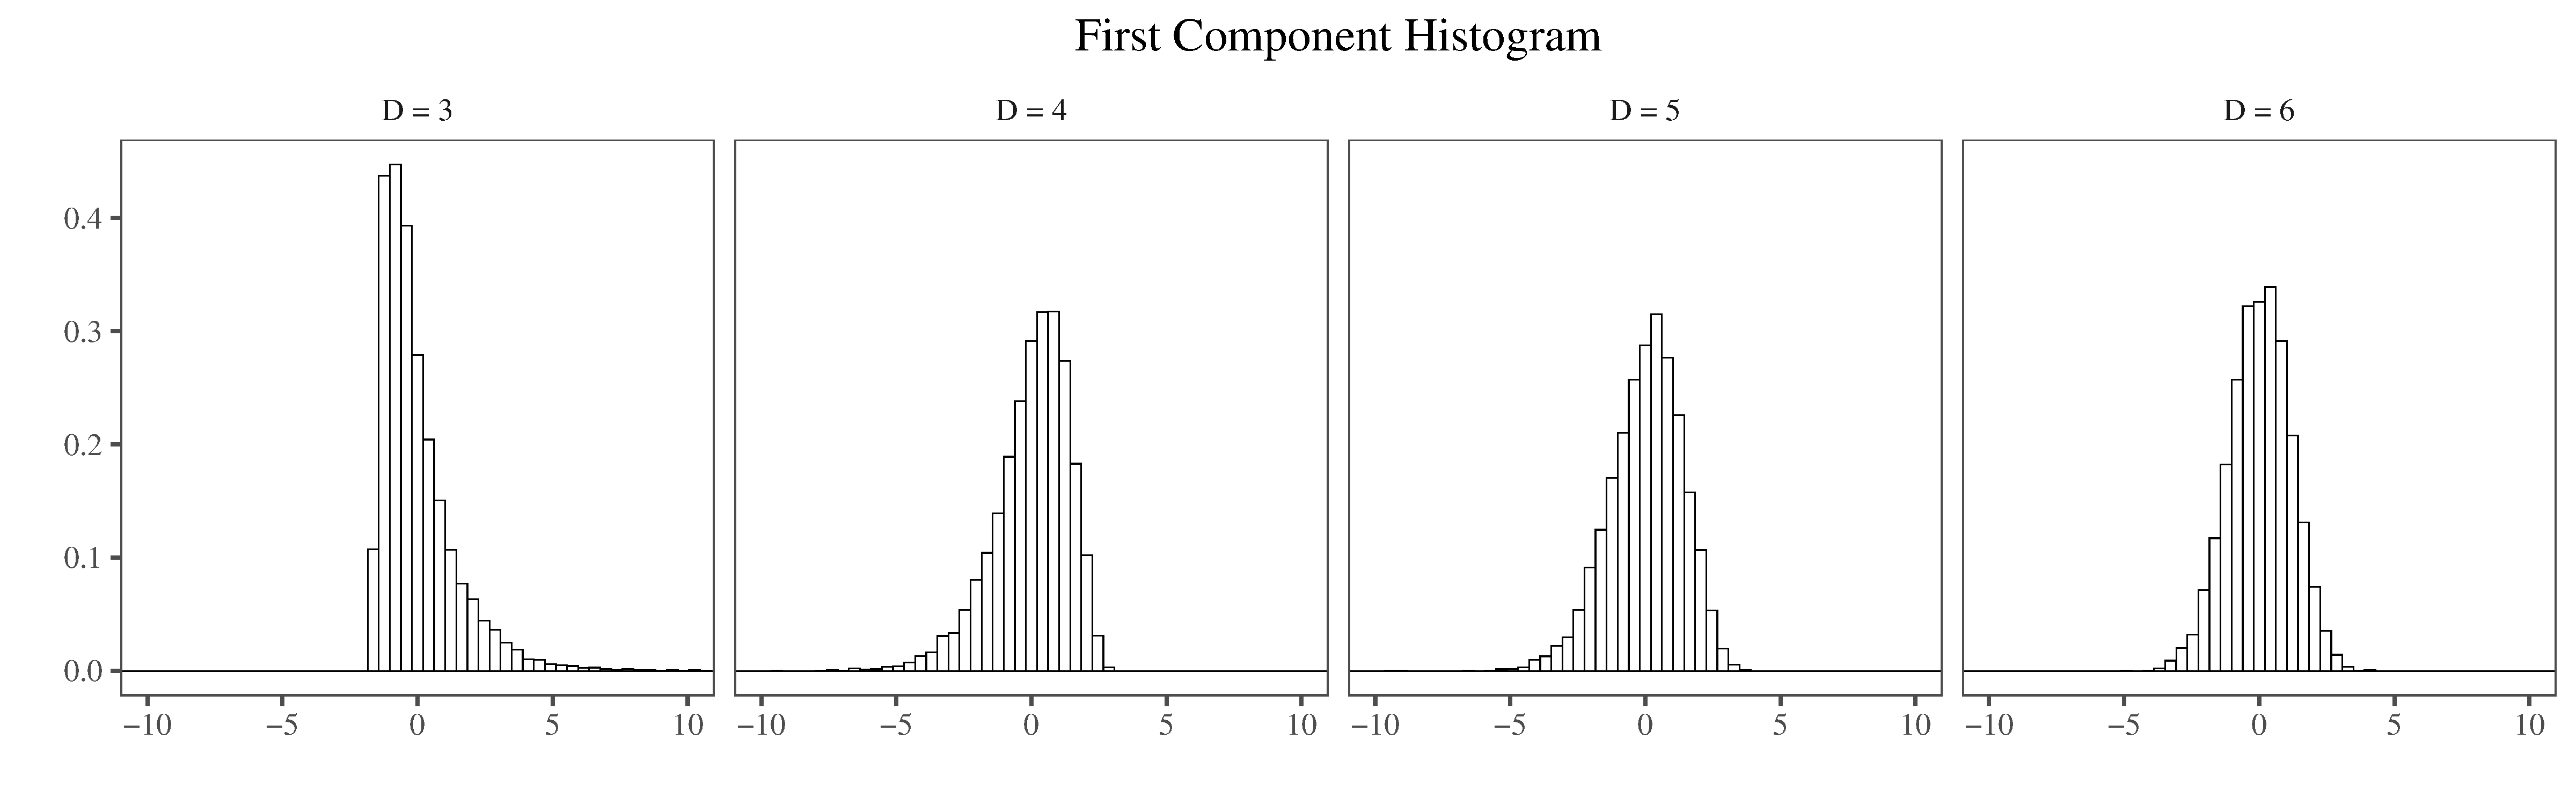
\includegraphics[width=\linewidth]{PCA-hist-50k}
	\caption{Histograms of the first principal component for $D=3,4,5,6$}
	\label{fig:PCA-Hist}
\end{figure}

\subsection{Test Size}

We assessed the size of the test by contrasting $100$ new TWNRS for each situation of $D=3,4,5,6$ and of $\alpha=0.01,0.05$.
Table~\ref{tab:result1} and Fig.~\ref{fig:RNG} 
show the results.

On the one hand, long series ($T=50000$) present a good size for every embedding dimension.
On the other hand, short series ($T=1000$) exhibit only one situation with a noticeable divergence between the expected and the observed size: the test rejects \SI{13}{\percent} of the $100$ series when $D=6$. 
In contrast, we expected \SI{1}{\percent} of rejection.
This might be because, in this case, the condition $D!\ll T$ is not respected.
Notice that the wrongly rejected TWNRS are all close to the point $(1,0)$.

%
%For large series, $T = 50000$, the closest although we observed a small drop in the percentage of data present in the region with $\SI{99}{\percent}$ confidence, there was a significant increase in points in the region with $\SI{95}{\percent}$ confidence, showing between $\SI{90}{\percent}$ and $\SI{88}{\percent}$ of the points when we vary the embedding dimension.
%
%For short series, $T = 1000$, and $D = 3$ 
%the conficence region at $\SI{99}{\percent}$ contains exactly $\SI{99}{\percent}$.
%
%On the other hand, there was a very large loss of points located in the region with $\SI{95}{\percent}$ confidence as the dimension increased.
%A reasonable explanation for this event is given in the choice of the parameter itself.
%It is known by definition that $D! \ll N$, which does not happen for such a sample size, thus presenting many missing patterns that lead to an unrepresentative probability distribution.

\begin{table}[hbt]
	\centering
	\caption{Empirical sizes of the test}
	\label{tab:result1}
	\begin{tabular}{*{3}rr}
		\toprule
		\multicolumn{1}{c}{$N$} & \multicolumn{1}{c}{$D$} & \multicolumn{1}{c}{\SI{95}{\percent}} & \multicolumn{1}{c}{\SI{99}{\percent}}\\
		%& $p$-value\\
		\cmidrule(lr){1-1}
		\cmidrule(lr){2-2}
		\cmidrule(lr){3-3}
		\cmidrule(lr){4-4}
		1000 & 3 & $0.98$ & $1.00$\\
		& 4 & $0.98$ & $0.96$\\
		& 5 & $1.00$ & $0.94$\\
		& 6 & $0.97$ & $0.87$\\
		\cmidrule(lr){1-4} 
		50000 & 3 & $0.97$ & $0.96$\\
		%& $0.47856$\\
		& 4 & $0.94$ & $0.95$\\
		%& $0.47555$\\ 
		& 5 & $0.97$ & $0.96$\\ 
		%& $0.48512$\\ 
		& 6 & $0.98$ & $0.99$\\ 
		%& $0.48058$\\
		\bottomrule
	\end{tabular}
\end{table}

\begin{figure}[hbt]
	\centering
	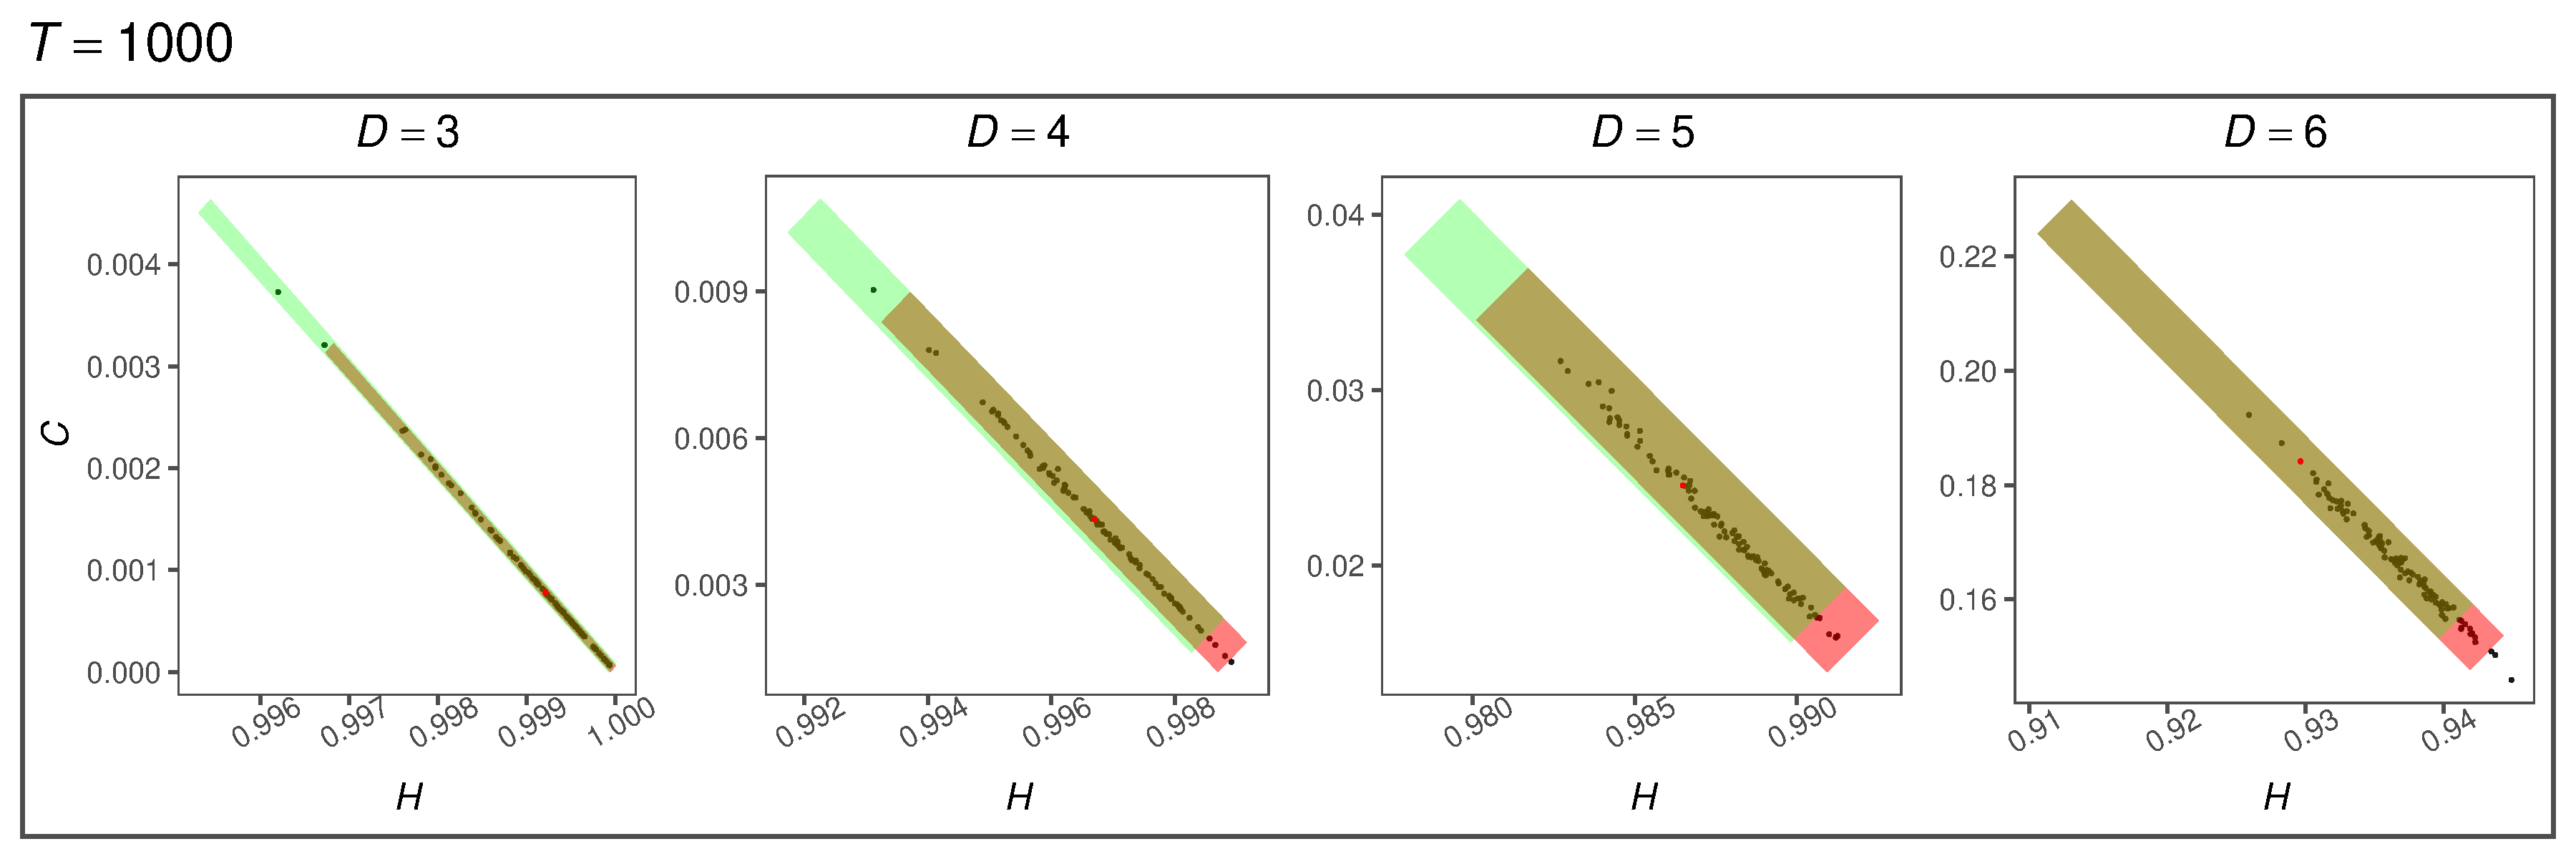
\includegraphics[width=\linewidth]{Figures/RNG-1000.pdf}
	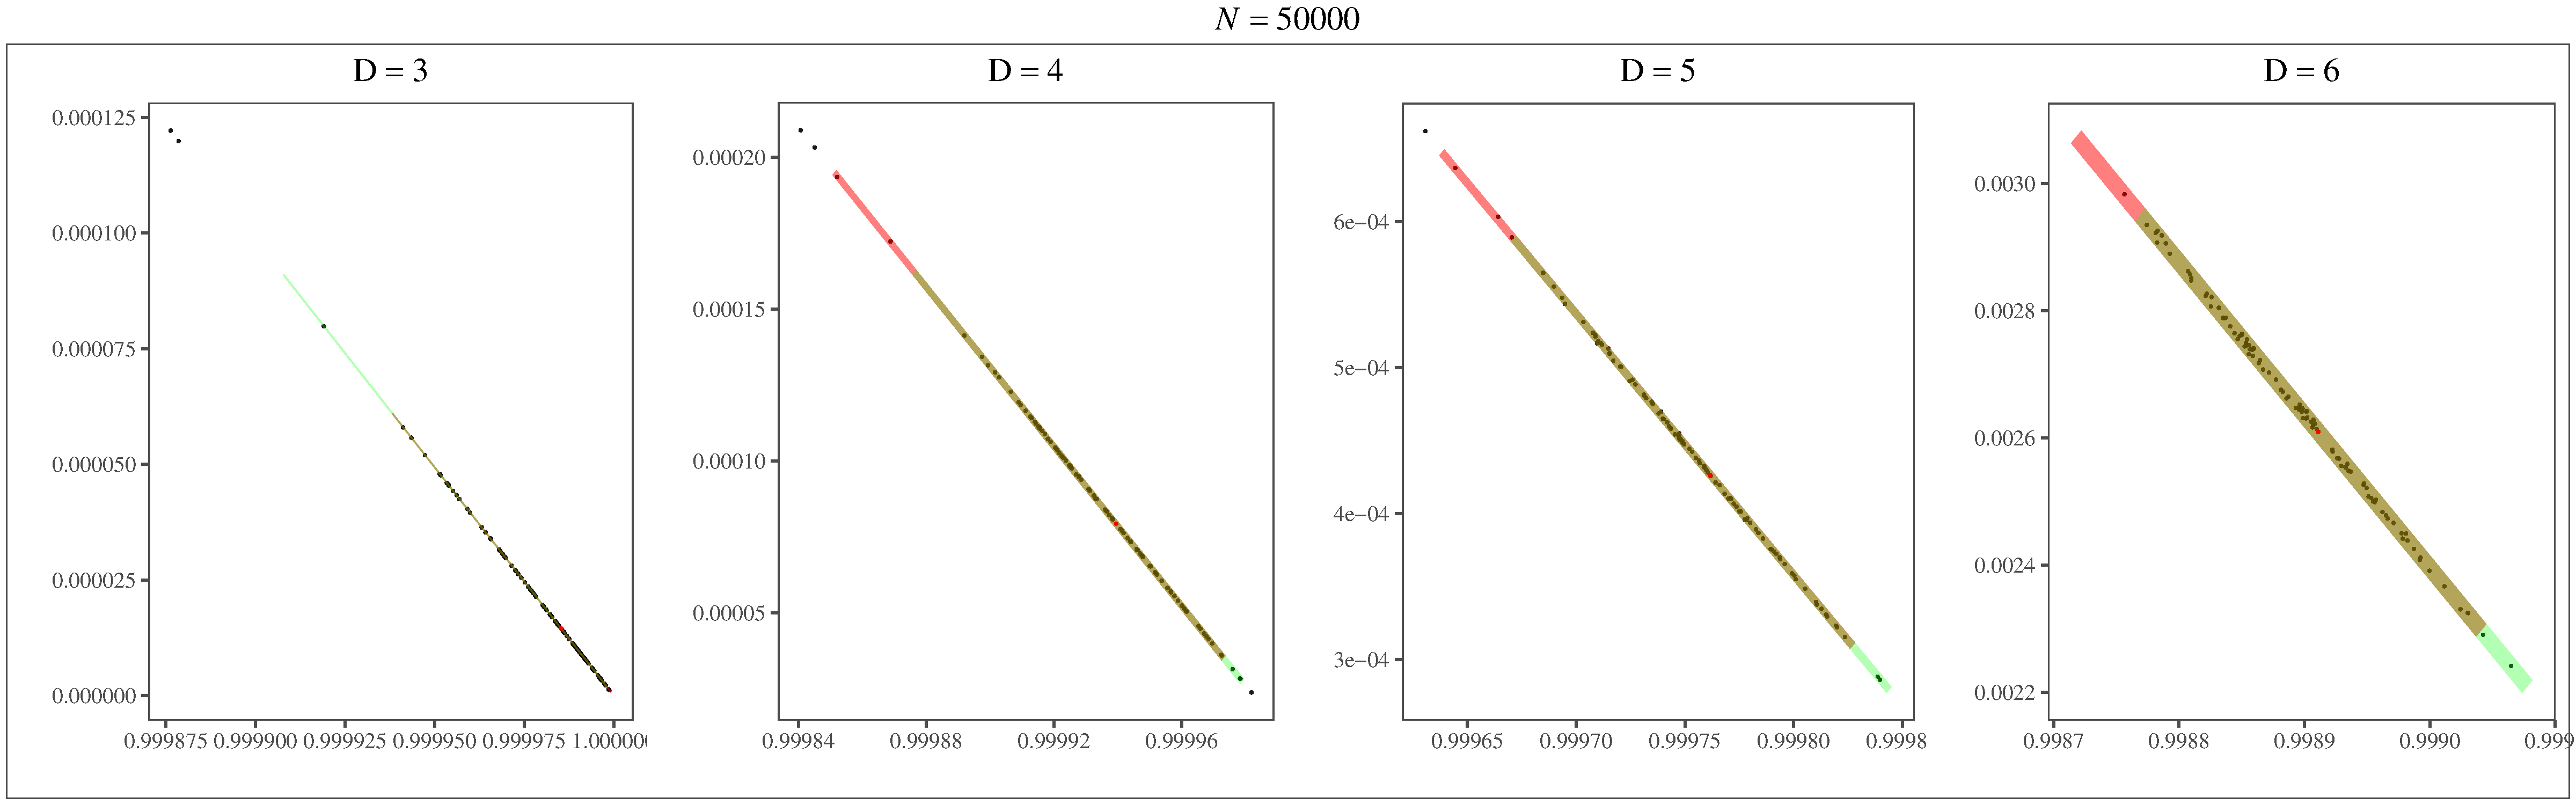
\includegraphics[width=\linewidth]{Figures/RNG-50000.pdf}
	\caption{New $100$ TRWNS and confidence regions.}
	\label{fig:RNG}
\end{figure}

We may then conclude that the test has good empirical size, provided $D!\ll T$, a condition that does not hold for $D=6$ and $T=1000$.


\subsection{Test Power}

\subsubsection{$H_1$: Correlated Noise}

We assessed the power of the test by contrasting time series with different correlation structure (under the $f^{-k}$ model) in the $H \times C$ plane.
Several studies in the literature have used this approach for identifying and characterizing randomness.

Our study's basis is the emblematic time series for each length $T$ and dimension embedding $D$.
Recall that the emblematic time was chosen as the most representative of the data set.
We use these series, transform them into $f^{-k}$ correlated noise, and verify the new point's location in the $H\times C$ plane.

%Fig.~\ref{fig:CorrNoisea} illustrates the effect of a white noise time series when adding correlation structures related to the $f^{-k}$ series for $k \in \{0, 1, 2, 3 \}$.
As we can observe in the plane, as the correlation between the observations increases, that is, $k > 0$, the randomness decreases, and the entropy presented decreases, informing the loss of its stochastic characteristic.

Fig.~\ref{fig:CorrNoisea} shows the overall effect of transforming the emblematic time series into $f^{-k}$ correlated noise, with $k=1/2,1,3/2,2,5/2,3$.
At this scale, the emblematic time series $k=0$ and the one with $k=1/2$ appear overlapped.
As the correlation increases with $k$, the randomness decreases, causing a drop in the entropy; the series become progressively more predictable.

Fig.~\ref{fig:CorrNoiseb} is a zoom close to the $(1,0)$ point, along with the confidence regions for the white noise.
We see that $ k = 0 $ and $ k = 0.1 $ are inside the $\SI{95}{\percent}$ confidence region, and $ k = 0.2 $ is inside the $\SI{99}{\percent}$ box.
Notice that the time series with $k=3/10$ is outside the confidence regions and does not pass the randomness test.
The same holds for all $k>3/10$.

\begin{figure}
	\centering
	\subfloat[Points in the $H\times C$ plane of the emblematic white noise  ($k=0$) and its transformations to become $f^{-k}$ correlated noise with $k=1/2,1,3/2,2,5/2,3$.\label{fig:CorrNoisea}]{
		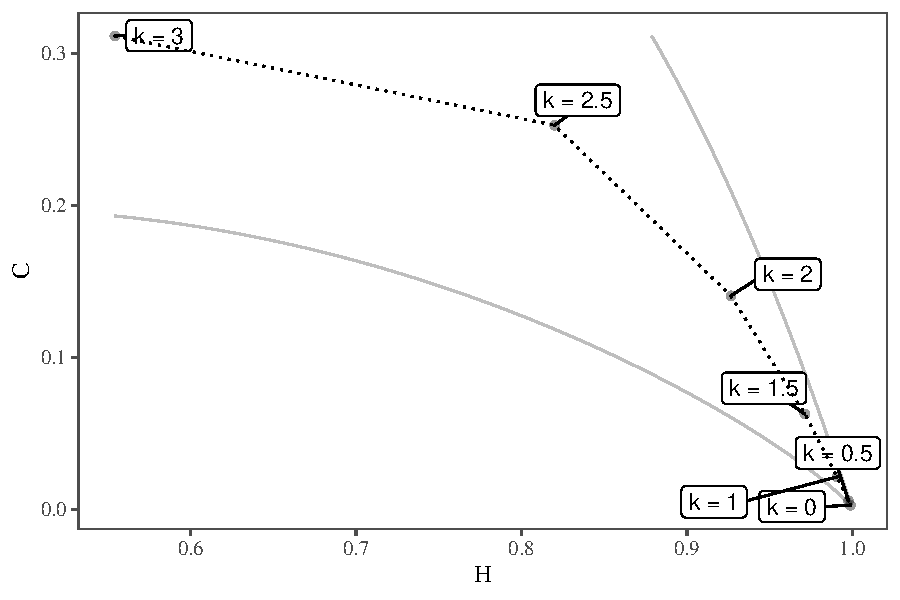
\includegraphics[width=.48\linewidth]{Figures/Correlation-Analysis-dotted.pdf}}
	\subfloat[Points of the emblematic white noise ($k=0$), and its $f^{-k}$ correlated noise versions, with $k=1/10, 1/5,3/10$ along with the confidence regions for white noise.\label{fig:CorrNoiseb}]{
		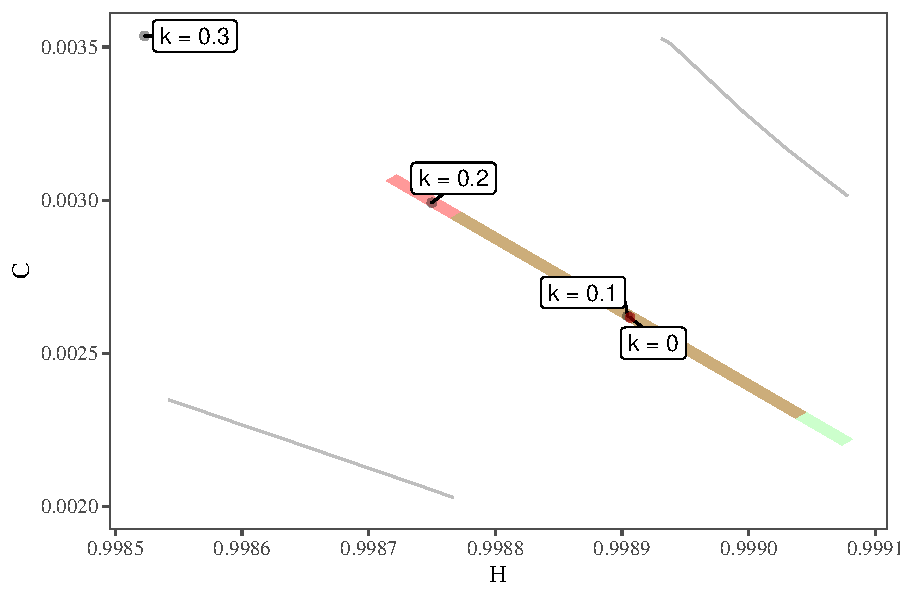
\includegraphics[width=.48\linewidth]{Figures/Correlation-Analysis-point.pdf}}
	\caption{Analysis of the test power with correlated $f^{-k}$ noise.}
	\label{fig:correlation}
\end{figure}

\subsubsection{$H_1$: Patch of Deterministic Function}

Consider the times series of length $T$ comprised of $T-[c100]$ white noise observations $x_1,x_2,\dots, x_{T-[c100]}$ followed by the signal $y_{T-[c100]+1}, y_{T-[c100]+2}, \dots, y_T$, in which $0\leq c \ll 1$ is the percentage of contamination.
We will verify the behavior of our test for the case $T=1000$, and $y_t$ an increasing function on $t$.
Fig.~\ref{Fig:PointsPatchedIncreasingFunction} shows the effect of such a contamination on the white noise time series whose point in the $H\times C$ plane appears in black.
The Figure also shows the confidence region at \SI{99}{\percent}.

\begin{figure}[hbt]
	\centering
	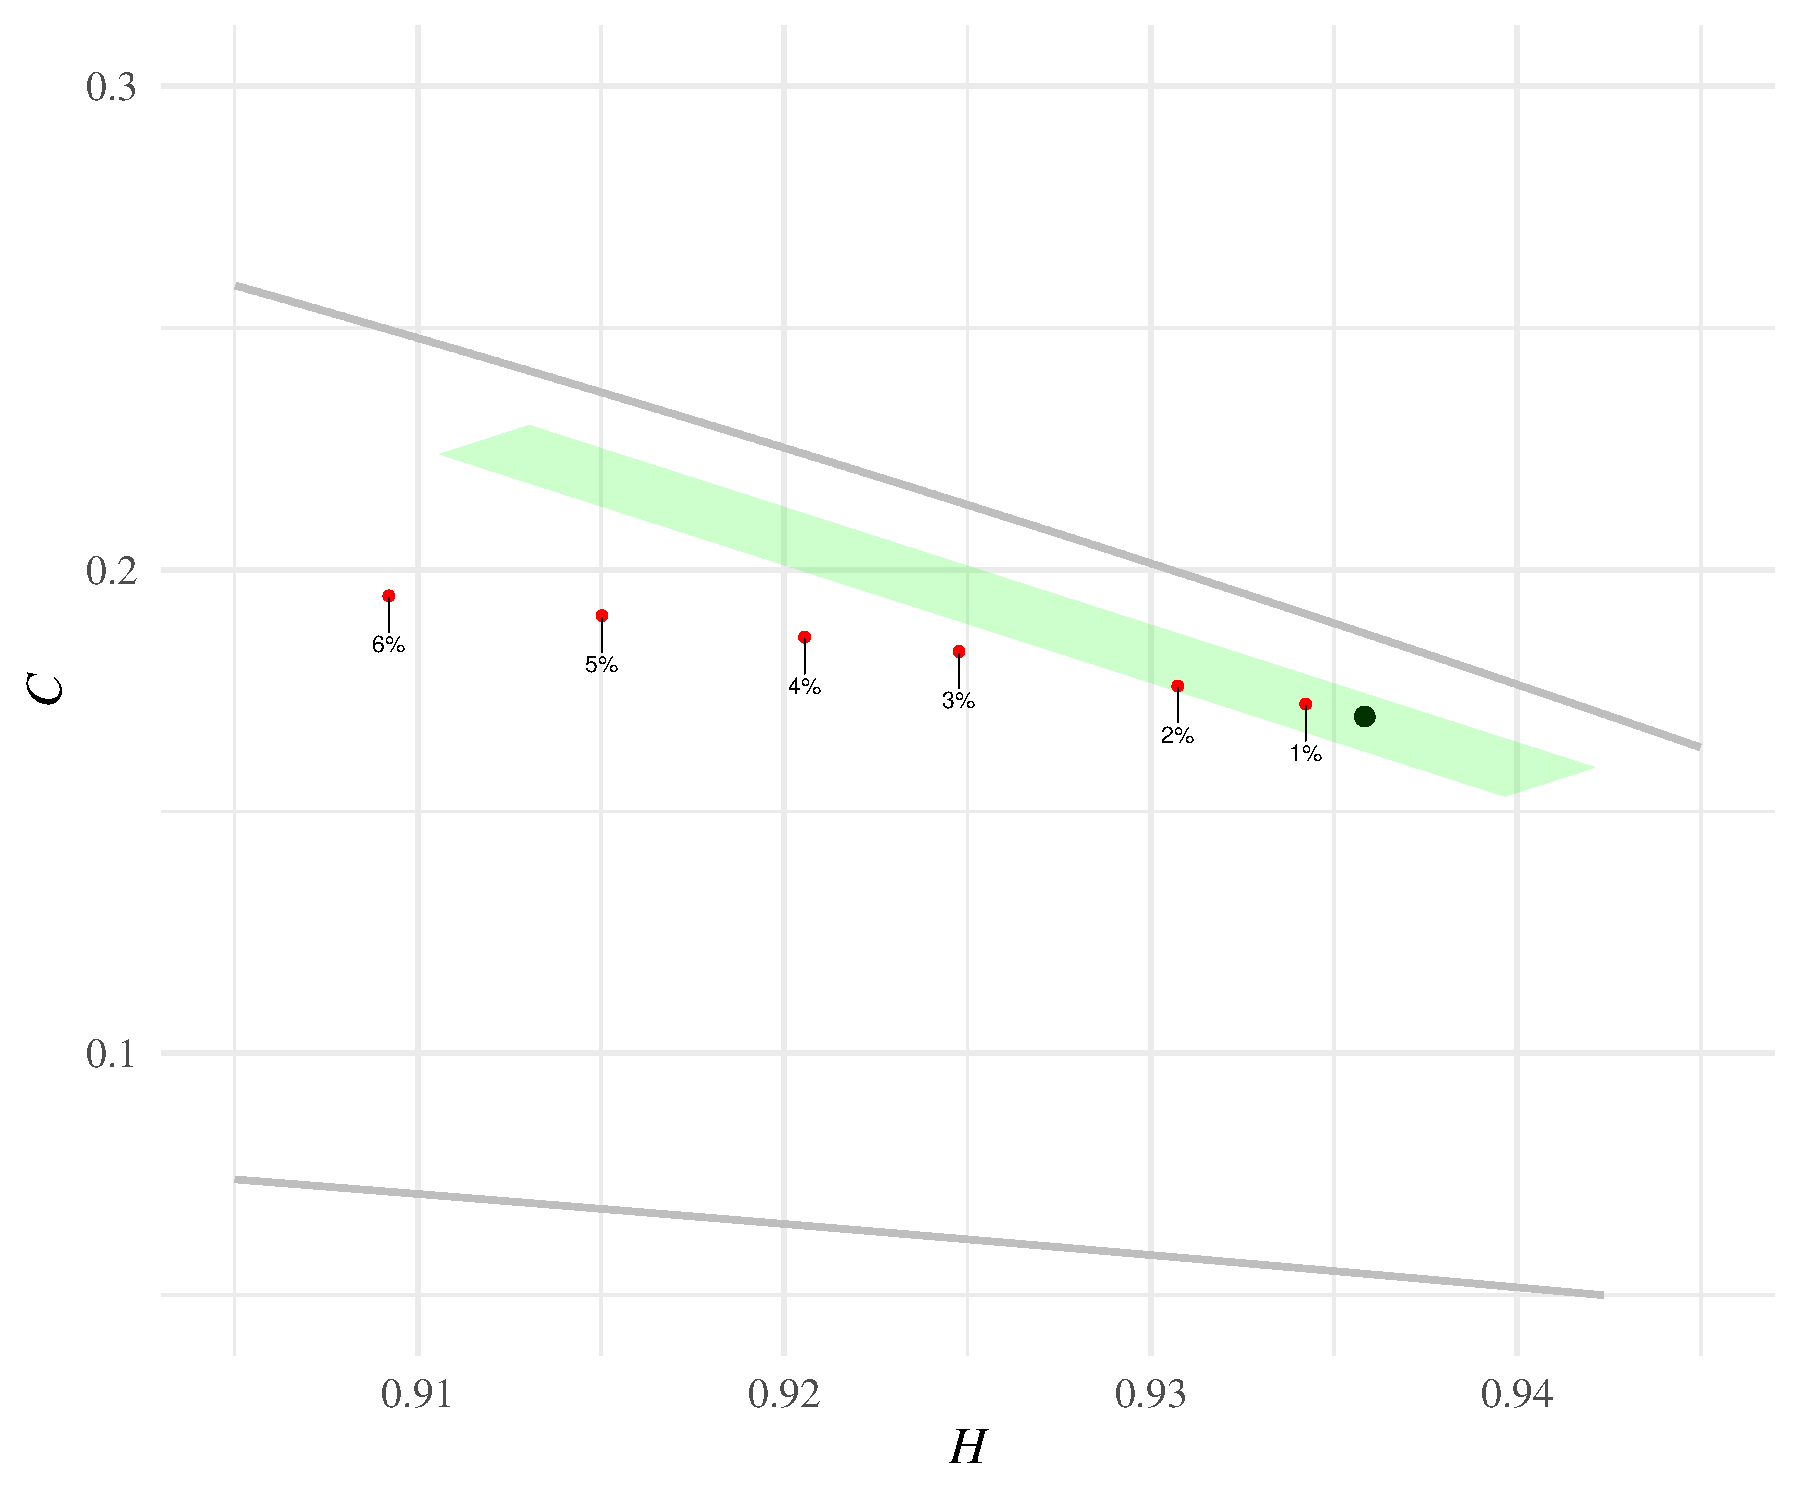
\includegraphics[width=.7\linewidth]{Figures/PointsPatchedIncreasingFunction}
	\caption{Effect of patching an increasing function at different levels to a white noise sequence.}\label{Fig:PointsPatchedIncreasingFunction}
\end{figure}
%%% The code that produces this figure starts at line 221, file "container_function.R"

The original point is displaced, at all levels of contamination, to a region with smaller entropy and larger complexity.
When the percentage of contamination is below approximately \SI{2}{\percent}, the test will not reject the null hypothesis at the \SI{99}{\percent}; in fact, the $p$-value is of around \SI{1.5}{\percent} for $c=0,0.01,0.02$.
The $p$-value falls to orders of $10^{-6}$ when the contamination is of \SI{3}{\percent} and above.

It is worth noticing that a test based solely on the entropy would have less power.
In this case, the complexity component enables the test to reject the null hypothesis at small contamination percentages.

\subsection{Revisiting the White Noise Hypothesis in the Literature}

In this section, we compare the performance of our test with that of 
previous analyses that employ the Entropy-Complexity plane.
To this aim, we produced $100$ sequences of length $T = \num[scientific-notation=true]{5 e4}$ for each generator and computed the $p$-value for each $D = \{3, 4, 5, 6\}$.
Previous results are shown in Table~\ref{Tab:Literature}, and ours are in Table~\ref{Tab:LiteratureComparations}.
We grouped our results in those that rejected (R) the null hypothesis and those that did not reject it (NR).

\begin{table}
	\caption{Results of the sequences generated by the main PRNGs in the literature. 
		The sequences have length $T=\num[scientific-notation = true]{5 e4}$.}
	\label{Tab:LiteratureComparations}
	\centering
	\begin{tabular}{cccc}
		\toprule
		Algorithm & 
		\multicolumn{1}{c}{$D$} & 
		$p$-value &
		HC-PCA\\
		\cmidrule(lr){1-1}
		\cmidrule(lr){2-2}
		\cmidrule(lr){3-3}
		\cmidrule(lr){4-4}
		MOT & 3 & 0.305 & NR\\
		& 4 & 0.572 & NR\\ 
		& 5 & 0.455 & NR\\ 
		& 6 & 0.508 & NR\\ 
		\cmidrule(lr){1-4}
		MWC & 3 & 0.501 & NR\\
		& 4 & 0.477 & NR\\ 
		& 5 & 0.496 & NR\\ 
		& 6 & 0.496 & NR\\ 
		\cmidrule(lr){1-4}
		COM & 3 & 0.123 & NR\\
		& 4 & 0.002 & R\\ 
		& 5 & \num[scientific-notation=true]{1.11 e-16} & R\\ 
		& 6 & \num[scientific-notation=true]{1.11 e-16} & R\\ 
		\cmidrule(lr){1-4}
		LEH & 3 & 0.531 & NR\\
		& 4 & 0.515 & NR\\ 
		\bottomrule
	\end{tabular}
	\begin{tabular}{|cccc}
		\toprule
		Algorithm & 
		\multicolumn{1}{c}{$D$} & 
		$p$-value &
		HC-PCA\\
		\cmidrule(lr){1-1}
		\cmidrule(lr){2-2}
		\cmidrule(lr){3-3}
		\cmidrule(lr){4-4}
		LEH & 5 & 0.495 & NR\\ 
		& 6 & 0.501 & NR\\ 
		\cmidrule(lr){1-4}
		fGn & 3 & 0.521 & NR\\
		& 4 & 0.519 & NR\\ 
		& 5 & 0.498 & NR\\ 
		& 6 & 0.470 & NR\\
		\cmidrule(lr){1-4}
		%fBm & 3 & \num[scientific-notation=true]{1.11 e-16} & R\\ 
		%& 4 & \num[scientific-notation=true]{1.11 e-16} & R\\ 
		%& 5 & \num[scientific-notation=true]{1.11 e-16} & R\\ 
		%& 6 & \num[scientific-notation=true]{1.11 e-16} & R\\ 
		%\cmidrule(lr){1-4}
		$f^{-k}$ & 3 & 0.482 & NR\\
		& 4 & 0.520 & NR\\ 
		& 5 & 0.513 & NR\\ 
		& 6 & 0.508 & NR\\
		\cmidrule(lr){1-4}
		LCG & 3 & 0.009 & R\\ 
		& 4 & \num[scientific-notation=true]{1.11 e-16} & R\\ 
		& 5 & \num[scientific-notation=true]{1.11 e-16} & R\\ 
		& 6 & \num[scientific-notation=true]{1.11 e-16} & R\\ 
		\bottomrule
	\end{tabular}
\end{table}

Comparing Tables~\ref{Tab:Literature} and~\ref{Tab:LiteratureComparations}, we see that our test captures adequately the random dynamics of the sequences produced by most of the analyzed generators.

It is noteworthy that the generator Combo RNG sequences only pass our white noise test for $D = 3$.
In higher embedding dimensions, as we consider longer words, the sequences produced by this generator are not labeled as white noise.

\section{Conclusions}\label{Sec:Conclusions}

We presented and evaluated the first test for white noise in the  Entropy-Complexity plane.
Our proposal is based on two stages:
(1)~building nonparametric empirical confidence regions in the principal components space and mapping these boxes back to the $H\times C$ plane.
(2)~computing an approximate $p$-value for a given sample by comparing it with points produced by true white noise random sequences (TWNRS).
We obtained the TWNRS with data from physical devices.

Our test has a good size, mostly with long TWNRS.
We also determined the power of our test for the alternative hypothesis of correlated $f^{-k}$ noise and found that it rejects the null hypothesis ($k=0$) for $k>3/10$.

Although our work focuses on the study of short sequences, we were able to capture the random behavior of well-known pseudorandom number generators already analyzed in the literature. 
With this, we verified the adequacy of our technique as it is capable of detecting correlation structures.

\section{Reproducibility and Replicability}\label{Sec:code}

Following the recommendations provided by \cite{ABadgingSystemforReproducibilityandReplicabilityinRemoteSensingResearch}, we make the text, source code, and data used in this study available at the \textit{Confidence-Regions} repository \url{https://github.com/EduardaChagas/ConfidenceRegions}.

\section{Acknowledgements}\label{Sec:acknowledgements}

This work was partially funded by the Coordination for the Improvement of Higher Education Personnel (CAPES) and National Council for Scientific and Technological Development (CNPq).

\printendnotes

\bibliography{References}

\end{document}